% Describir el diseño o el planteamiento que ha sido utilizado para el desarrollo del componente, el cual depende del método seleccionado (hipotético-deductivo, inductivo, entre otros). Se sugiere incluir, los que correspondan:

% \begin{itemize}
%     \item Enfoque (cualitativo, cuantitativo o mixto).
%     \item Tipo de trabajo: exploratorio, descriptivo, explicativo, experimental, estudio de casos, entre otros.
%     \item Técnica de recolección de información (entrevistas, cuestionarios, análisis documental, entre otras).
%     \item Técnica de análisis de la información.
% \end{itemize}

% Este capítulo debe incluir toda la información necesaria para que un interesado pueda replicar el componente sin dificultades. Se debe mencionar explícitamente cuáles actividades se realizaron para cumplir con los objetivos planteados.

Para el desarrollo del proyecto se hizo uso de SCRUM \cite{SCRUM} como marco de trabajo a través de 4 sprints \cite{SCRUM-Sprints} (Tomando en cuenta el Sprint 0). Cada subsección representa un Sprint en concreto. 

%%%%%%%%%%%%%%%%%%%%%%%%%%%%%%%%%%%%%%%%%%%
%--------------- SPRINT 0 ---------------%
%%%%%%%%%%%%%%%%%%%%%%%%%%%%%%%%%%%%%%%%%%%
\section{Sprint 0}
\label{chapter02-section02-sprint0}
En este sprint denominado el \textit{"Sprint 0"}, se definieron aspectos fundamentales para el éxito del proyecto, con el objetivo de preparar al equipo y el entorno para los sprints de desarrollo regulares. 

\begin{itemize}
    \item Se realizó un análisis exhaustivo del stack tecnológico que se usará para el desarrollo, tanto del lado del frontend como del backend, abordando cada uno de los dos backends (ResNet Y ResearchDecide) y los cuatro componentes diferentes del sistema, los cuales son:
    \begin{itemize}
        \item Automatización del proceso de extracción, depuración y almacenamiento de datos de Scopus mediante la API de Elsevier.
        \item Desarrollo de módulo que implemente funciones del tipo red social para los usuarios del sistema.
        \item Implementación de estrategia(s) de mediación o facilitación del consenso (sistema como mediador para el grupo de investigadores).
        \item Desarrollo del módulo de Analítica: Dashboards y estadísticas para la toma de decisiones.
    \end{itemize}
    El propósito de este análisis es garantizar que tanto el frontend como el backend utilicen las tecnologías más apropiadas para satisfacer los requisitos técnicos y de negocio; y así, asegurar, y para así asegurar una integración efectiva y eficiente entre todas las partes del sistema.
    

    En consecuencia, se tomaron las siguientes decisiones:
    \begin{enumerate}
        \item Para la integración del sistema  en el lado del frontend se optó por utilizar Angular como framework de desarrollo, debido a que se puede reutilizar componentes de el sistema ResNet \cite{RESNET}. 
        \item Para el lado del backend se propuso utilizar Django como framework. Con Django, se espera aprovechar su robustez, seguridad y su capacidad para desarrollar rápidamente aplicaciones web escalables y de alto rendimiento. Además, Django ofrece una amplia gama de características integradas, como autenticación de usuarios, administración de bases de datos, y un ORM\footnote{ORM (Object-Relational Mapping) es una herramienta que facilita la comunicación y traducción de datos entre bases de datos relacionales y objetos en programación orientada a objetos.} potente, lo que lo hace una elección sólida para el desarrollo del backend del sistema. 
        \item Para mantener las mismas dependencias de desarrollo y simplificar la gestión del entorno, se utilizará Docker \cite{DOCKER}. Esto permite encapsular aplicaciones y sus dependencias en contenedores, asegurando consistencia entre entornos.
        \item Además, Docker Compose se empleará para orquestar el servidor backend y la base de datos, facilitando la configuración y gestión del entorno, y simplificando el despliegue del sistema en diferentes entornos.
        \item La elección de Neo4j se basa en la decisión de no alterar el modelo de datos actual. Dado que Neo4j está especialmente diseñado para modelos de datos conectados y relacionales, su adopción evita la necesidad de reestructurar el modelo existente, ahorrando tiempo y recursos mientras garantiza la continuidad del desarrollo del sistema.
        \item El control de versiones se hará mediante Git y para alojar dichas versiones se utilizará GitHub. Mediante una organización en donde se alojará el código fuente de los 4 componentes.
        \item Para la gestión del proyecto, se utilizó SCRUM en conjunto con Azure DevOps \cite{AZURE-DEVOPS}. SCRUM proporciona un marco ágil para la planificación y ejecución de proyectos, mientras que Azure DevOps \cite{AZURE-DEVOPS} ofrece herramientas integradas para facilitar todas las etapas del ciclo de vida del desarrollo de software. Esta combinación garantiza una gestión eficiente y colaborativa del proyecto, mejorando la transparencia y la entrega oportuna de resultados.
        En la Figura \ref{fig:azure-devops-project} se muestra el proyecto en Azure DevOps.
        \begin{figure}[H]
            \centering
            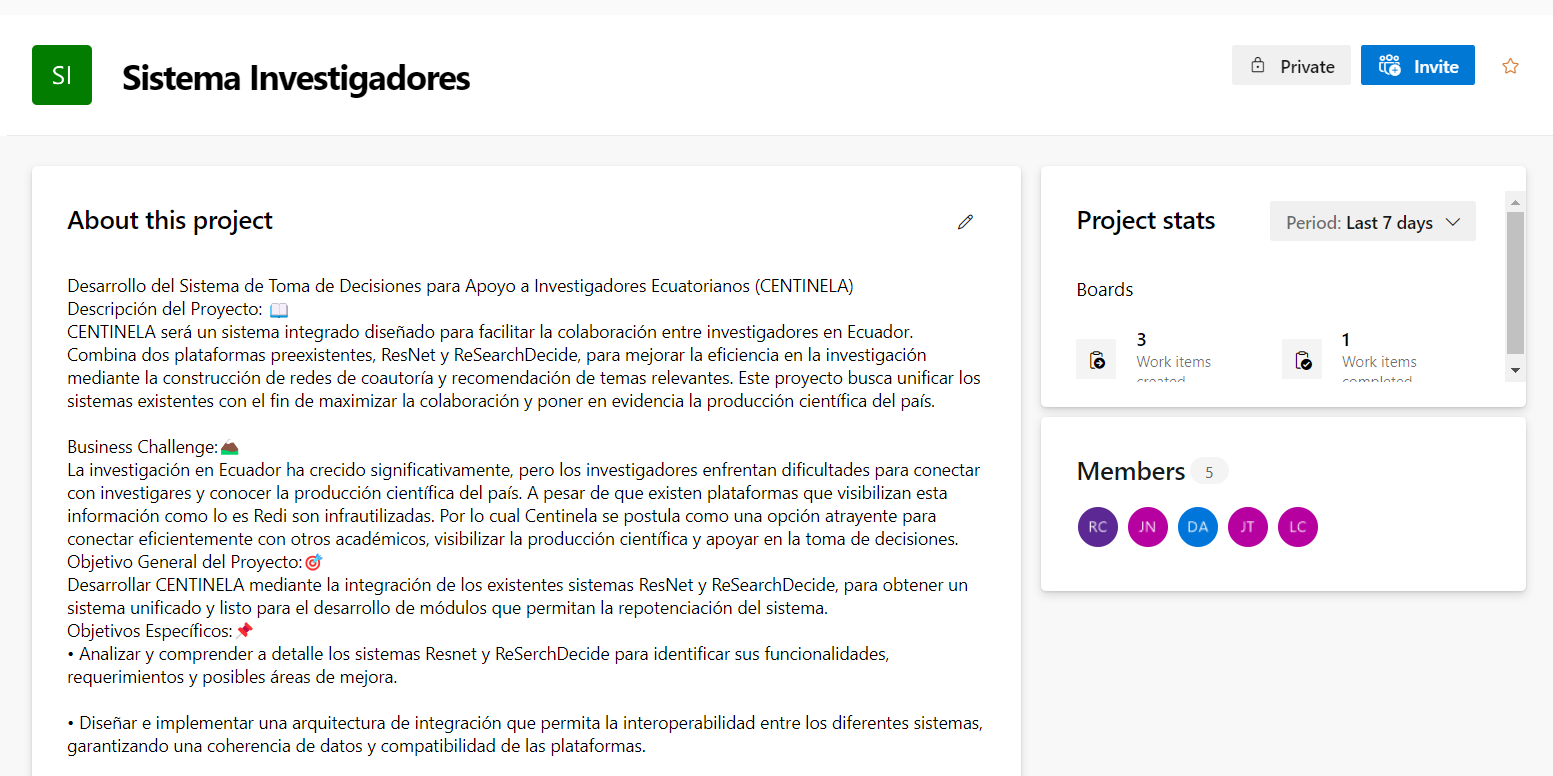
\includegraphics[width=0.5\linewidth]{../02Figures//02Chapter//Sprints//Sprint-0/azure-devops-project.png}
            \caption{Proyecto en Azure DevOps}
            \label{fig:azure-devops-project}
        \end{figure}
        \item Se optó por Visual Studio Code como editor de código para el frontend y PyCharm como IDE de desarrollo especializado para el backend. Esta elección proporcionó un entorno flexible y eficaz para la colaboración en el proyecto.
    \end{enumerate}

    \item Se establecieron horarios para las reuniones diarias, las cuales se llevarán a cabo los días lunes, martes, miércoles y jueves en el horario de 14:00 a 16:00 en un espacio proporcionado por la directora del proyecto, Lorena Recalde, en el edificio de Sistemas-EPN. Durante este intervalo, se realizaron los daily meetings y se llevó a cabo el trabajo en equipo.

    \item Se  decidió adoptar el inglés como el idioma oficial para la codificación, los commits y toda la documentación técnica dentro de nuestro equipo. Esta medida busca estandarizar nuestras prácticas con los estándares internacionales, facilitar la colaboración con otros equipos y mejorar la accesibilidad a recursos técnicos de alta calidad.

    \item Se decidió utilizar Arquitectura Hexagonal \cite{ARQUITECTURA-HEXAGONAL} como patrón de arquitectura, definiendo así una estructura de carpetas y respetando los principios de esta arquitectura. Cabe destacar que no se ha implementado arquitectura hexagonal en su totalidad, ya que se optó por una adaptación de la misma, obteniendo así una arquitectura de dos capas.
    \begin{itemize}
        \item \textbf{Backend}: Para el backend, en cuanto a  la estructura de carpetas, se definió que por cada módulo en general se tendrá las tres  capas de arquitectura como son infraestructura, aplicación y dominio como se muestra en la Figura \ref{fig:hexagonal-architecture-example-backend}.

        \begin{figure}[H]
            \centering
            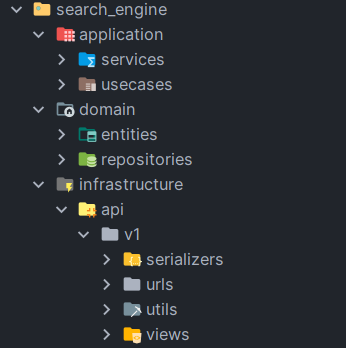
\includegraphics{../02Figures/02Chapter/Sprints/Sprint-0/hexagonal-architecture-example.png}
            \caption{Arquitectura Hexagonal aplicada en el modulo del motor de búsqueda}
            \label{fig:hexagonal-architecture-example-backend}
        \end{figure}
        \item \textbf{Frontend}: Basándonos en el concepto de puertos y adaptadores, en el frontend también hemos optado por  implementar la Arquitectura Hexagonal \cite{ARQUITECTURA-HEXAGONAL} como patrón de arquitectura, con algunas adaptaciones específicas para este contexto. Dado que el frontend se enfoca en la parte gráfica, el adaptador se denominará "presentación", donde se gestionará toda la interfaz gráfica. Esta capa de presentación será el punto de entrada hacia el núcleo (core) de la aplicación frontend, facilitando así una separación clara entre la lógica de negocio y la interfaz de usuario, y promoviendo una estructura modular y fácilmente mantenible (Figura \ref{fig:hexagonal-architecture-example-frontend}.)
        \begin{figure}[H]
            \centering
            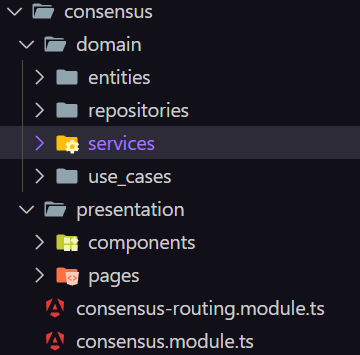
\includegraphics{../02Figures/02Chapter/Sprints/Sprint-0/hexagonal-architecture-example-frontend.png}
            \caption{Arquitectura hexagonal aplicada al modulo de consenso}
            \label{fig:hexagonal-architecture-example-frontend}
        \end{figure}
    \end{itemize}
\end{itemize}

%%%%%%%%%%%%%%%%%%%%%%%%%%%%%%%%%%%%%%%%%%%
%--------------- SPRINT 1 ---------------%
%%%%%%%%%%%%%%%%%%%%%%%%%%%%%%%%%%%%%%%%%%%
\section{Sprint 1}
\label{chapter02-section02-sprint1}
\subsection{Introducción}
Durante este sprint, nuestro objetivo principal es crear diseños detallados que integren las funcionalidades de las aplicaciones Resnet (ver Sección \ref{chapter01-section03:ResNet}) y Research Decide en una plataforma unificada. Además, nos centraremos en identificar y proponer mejoras significativas para esta aplicación combinada. Utilizaremos Figma para desarrollar los mockups, aplicando los patrones de diseño más adecuados para asegurar una experiencia óptima para el usuario final. Es importante destacar que esta fase será iterativa, permitiendo ajustes y cambios continuos durante todo el desarrollo, por lo que la propuesta final no será definitiva.
\subsection{Objetivos del Sprint}

\begin{itemize}
    \item Diseñar el flujo de navegación de la aplicación combinada.
    \item Crear mockups de las interfaces de usuario de la aplicación.
    \item Desarrollar la estructura  principal del motor de búsqueda.
    \item Implementar el enrutamiento de la aplicación.
    \item Implementar la página de inicio de la aplicación.
\end{itemize}
\subsection{Planificación}
Para este sprint, hemos seleccionado las historias de usuario con su respectivo código enfocadas principalmente en la integración gráfica de las plataformas mencionadas en la Sección \ref{chapter01-section03:ResNet}, que se muestran en la Tabla \ref{C2T1:Historias de Usuario del Sprint 1}. 
Se debe tomar en cuenta que esta parte del desarrollo se enfoca en los usuarios que no necesariamente están registrados en la plataforma, por lo que se ha priorizado la visualización de información relevante para estos usuarios.
\begin{table}[H]
    \centering
    \begin{tabular}{|m{2.5cm}|m{5cm}|m{6cm}|}
        \hline
        \textbf{Identificador} &  \textbf{Historia de Usuario} & \textbf{Tareas} \\
        
        \hline
        Visual Studio Code & Como usuario no registrado deseo poder encontrar artículos relevantes dado un  tema de investigación para poder acceder rápidamente a información útil y actualizada que apoye mi estudio o trabajo  &  
        \begin{itemize}
            \item Componente para listar \break artículos
            \item Paginación para extraer resultados limitados
            \item Componente para filtrar la información por años
            \item Enrutamiento para redirigir hacia la página del articulo
            \item Página para visualizar información general del articulo
            
        \end{itemize} 
        \\
        \hline
          Visual Studio Code & Como usuario no registrado deseo poder ver los investigadores que tengan colaboraciones en artículos con afiliaciones ecuatorianas para mantenerme informado sobre sus investigaciones y campos de estudio &  
        \begin{itemize}
            \item Componente para listar Artículos
            \item Paginación para extraer resultados limitados
            \item Componente para filtrar la información por años
            \item Enrutamiento para redirigir hacia  la página del Articulo
            \item Página para visualizar información general del Articulo
            
        \end{itemize} 
        \\
        \hline
        
    \end{tabular}
    \caption{Historias de Usuario del sprint 1}
    \label{C2T1:Historias de Usuario del Sprint 1}
\end{table}


Todas las historias de usuario se han dividido en tareas más pequeñas y manejables. 
También en las Figuras \ref{fig:aceptance-criteria-HU-SE-01}  y  \ref{fig:aceptance-criteria-HU-SE-02} se muestran los criterios de aceptación de cada historia de usuario, que se utilizarán para verificar si la historia de usuario se ha completado correctamente.
\begin{figure}[H]
    \centering
    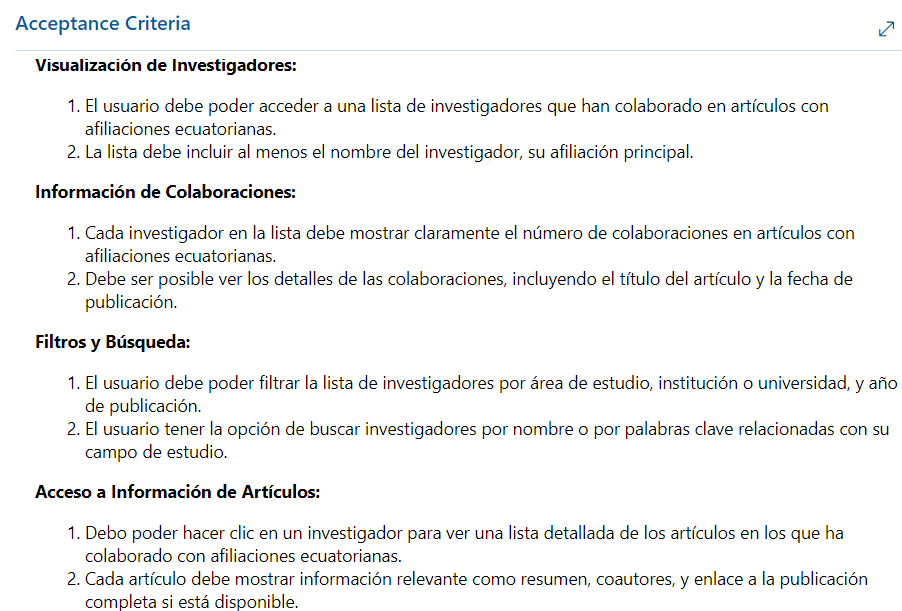
\includegraphics[scale=0.7]{../02Figures/02Chapter/Sprints/Sprint-1/aceptance-criteria-HU-SE-01.png}
    \caption{Criterios de aceptación de la historia de usuario HU-SE-01}
    \label{fig:aceptance-criteria-HU-SE-01}
\end{figure}
\begin{figure}[H]
    \centering
    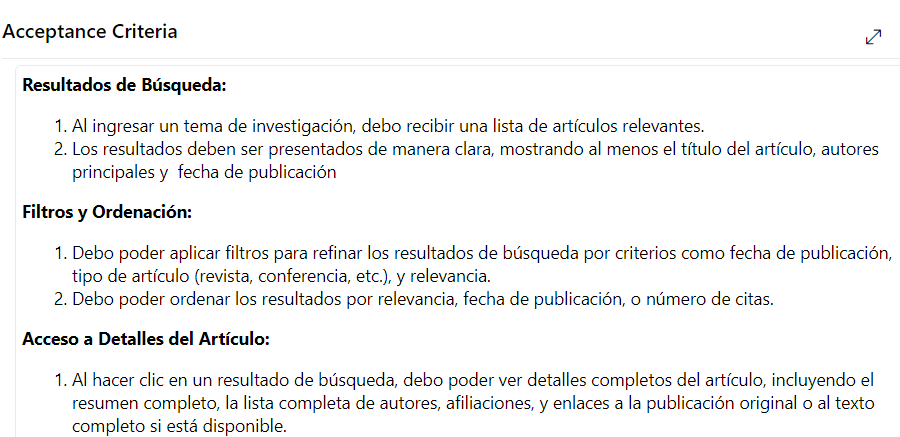
\includegraphics[scale=0.7]{../02Figures/02Chapter/Sprints/Sprint-1/aceptance-criteria-HU-SE-02.png}
    \caption{Criterios de aceptación de la historia de usuario HU-SE-02}
    \label{fig:aceptance-criteria-HU-SE-02}
\end{figure}


Estas historias de usuario se han priorizado en función de su importancia y complejidad, y se han asignado a los miembros del equipo de desarrollo. La Figura \ref{fig:azure-board-sprint-1} muestra las tareas asignadas a cada miembro del equipo.
\begin{figure}[H]
    \centering
    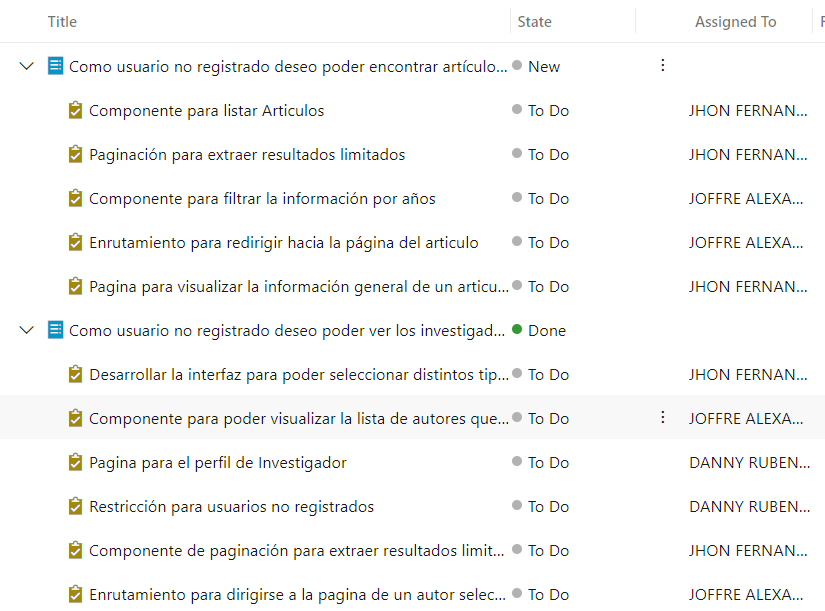
\includegraphics[scale=0.9]{../02Figures/02Chapter/Sprints/Sprint-1/fig_azure-board-sprint-1.png}
    \caption{Planificación de tareas del Sprint 1}
    \label{fig:azure-board-sprint-1}
\end{figure}

\subsection{Implementación}
Para la implementación de las historias de usuario, se ha utilizado la herramienta de diseño Figma, que permite crear prototipos de alta y baja fidelidad. 
A continuación, se presentan los mockups de las interfaces de usuario de la aplicación que se han desarrollado durante este sprint.
Cabe destacar que se siguió un proceso iterativo, por lo que los mockups presentados no son definitivos y pueden sufrir cambios en futuras iteraciones.
Además el diseño se baso en el patrón de diseño Mobile First \cite{MOBILE-FIRST}, que consiste en diseñar primero la versión móvil de la aplicación y luego adaptarla a dispositivos de mayor tamaño.

\subsubsection{Página de inicio}
La página de inicio de la aplicación es la primera pantalla que verá el usuario al ingresar a la plataforma. 
En esta pantalla, se mostrarán las opciones de búsqueda y un conjunto de datos sobre la información que tiene Centinela. Así como también una barra de navegación que permitirá al usuario acceder a otras secciones de la aplicación. 
La figura \ref{fig:mockup-home} muestra el diseño de la página de inicio.

\begin{figure}[H]
    \centering
    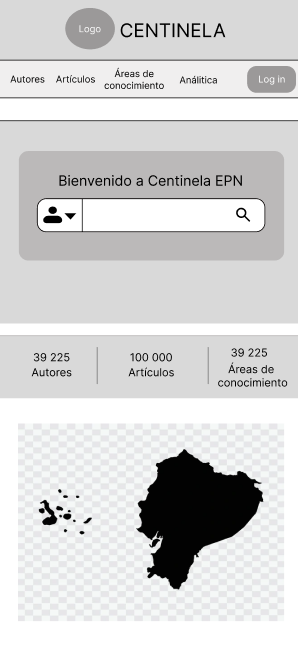
\includegraphics[scale=0.9]{../02Figures/02Chapter/Sprints/Sprint-1/mobile-first-home.png}
    \caption{Mockup de la página de inicio}
    \label{fig:mockup-home}
\end{figure}

Como se menciono en la sección \ref{chapter02-section02-sprint0} se utilizara una adaptación de arquitectura hexagonal para desarrollar la estructura de la aplicación.
Dando como resultado la estructura de carpetas que se muestra en la figura \ref{fig:hexagonal-architecture-home}.
Puesto que la página de inicio es la primera pantalla que verá el usuario al ingresar a la plataforma, se ha decidido crear una carpeta específica para esta sección.
También debido a que angular es un framework que se maneja con componentes, se ha creado un componente para la página de inicio, el cual se encuentra en la carpeta de pages.
A su vez  se ha creado el archivo de tipo module para la página de inicio, el mismo nos permitirá importar los componentes necesarios para la página de inicio, sin tener que importarlos en el archivo principal de la aplicación.
Este enfoque permitirá que el modulo de la página de inicio sea independiente del resto de la aplicación, que juntado con la arquitectura hexagonal facilitara la escalabilidad y mantenimiento de la aplicación.

\begin{figure}[H]
    \centering
    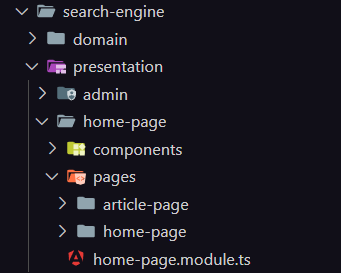
\includegraphics[scale=0.8]{../02Figures/02Chapter/Sprints/Sprint-1/home-page-ha.png}
    \caption{Estructura de carpetas de la página de inicio}
    \label{fig:hexagonal-architecture-home}
\end{figure}

Resultado de la implementación de la página de inicio se muestra en la figura \ref{fig:home-page}.
En la que se muestra la barra de navegación, el formulario de búsqueda y la información que tiene Centinela. El formulario de búsqueda cuenta con 3 opciones, 
la primera es para buscar por palabra clave a un autor, la segunda es para buscar autores relevantes dado un tópico de investigación y la tercera es para buscar artículos relevantes dado un tópico.
Bajo el motor de búsqueda se muestra el resumen del numero de artículos, autores y tópicos que tiene registrado Centinela.
Finalmente contiene un mapa que mostrará en que el número de artículos que se han publicado en cada provincia del Ecuador.
\begin{figure}[H]
    \centering
    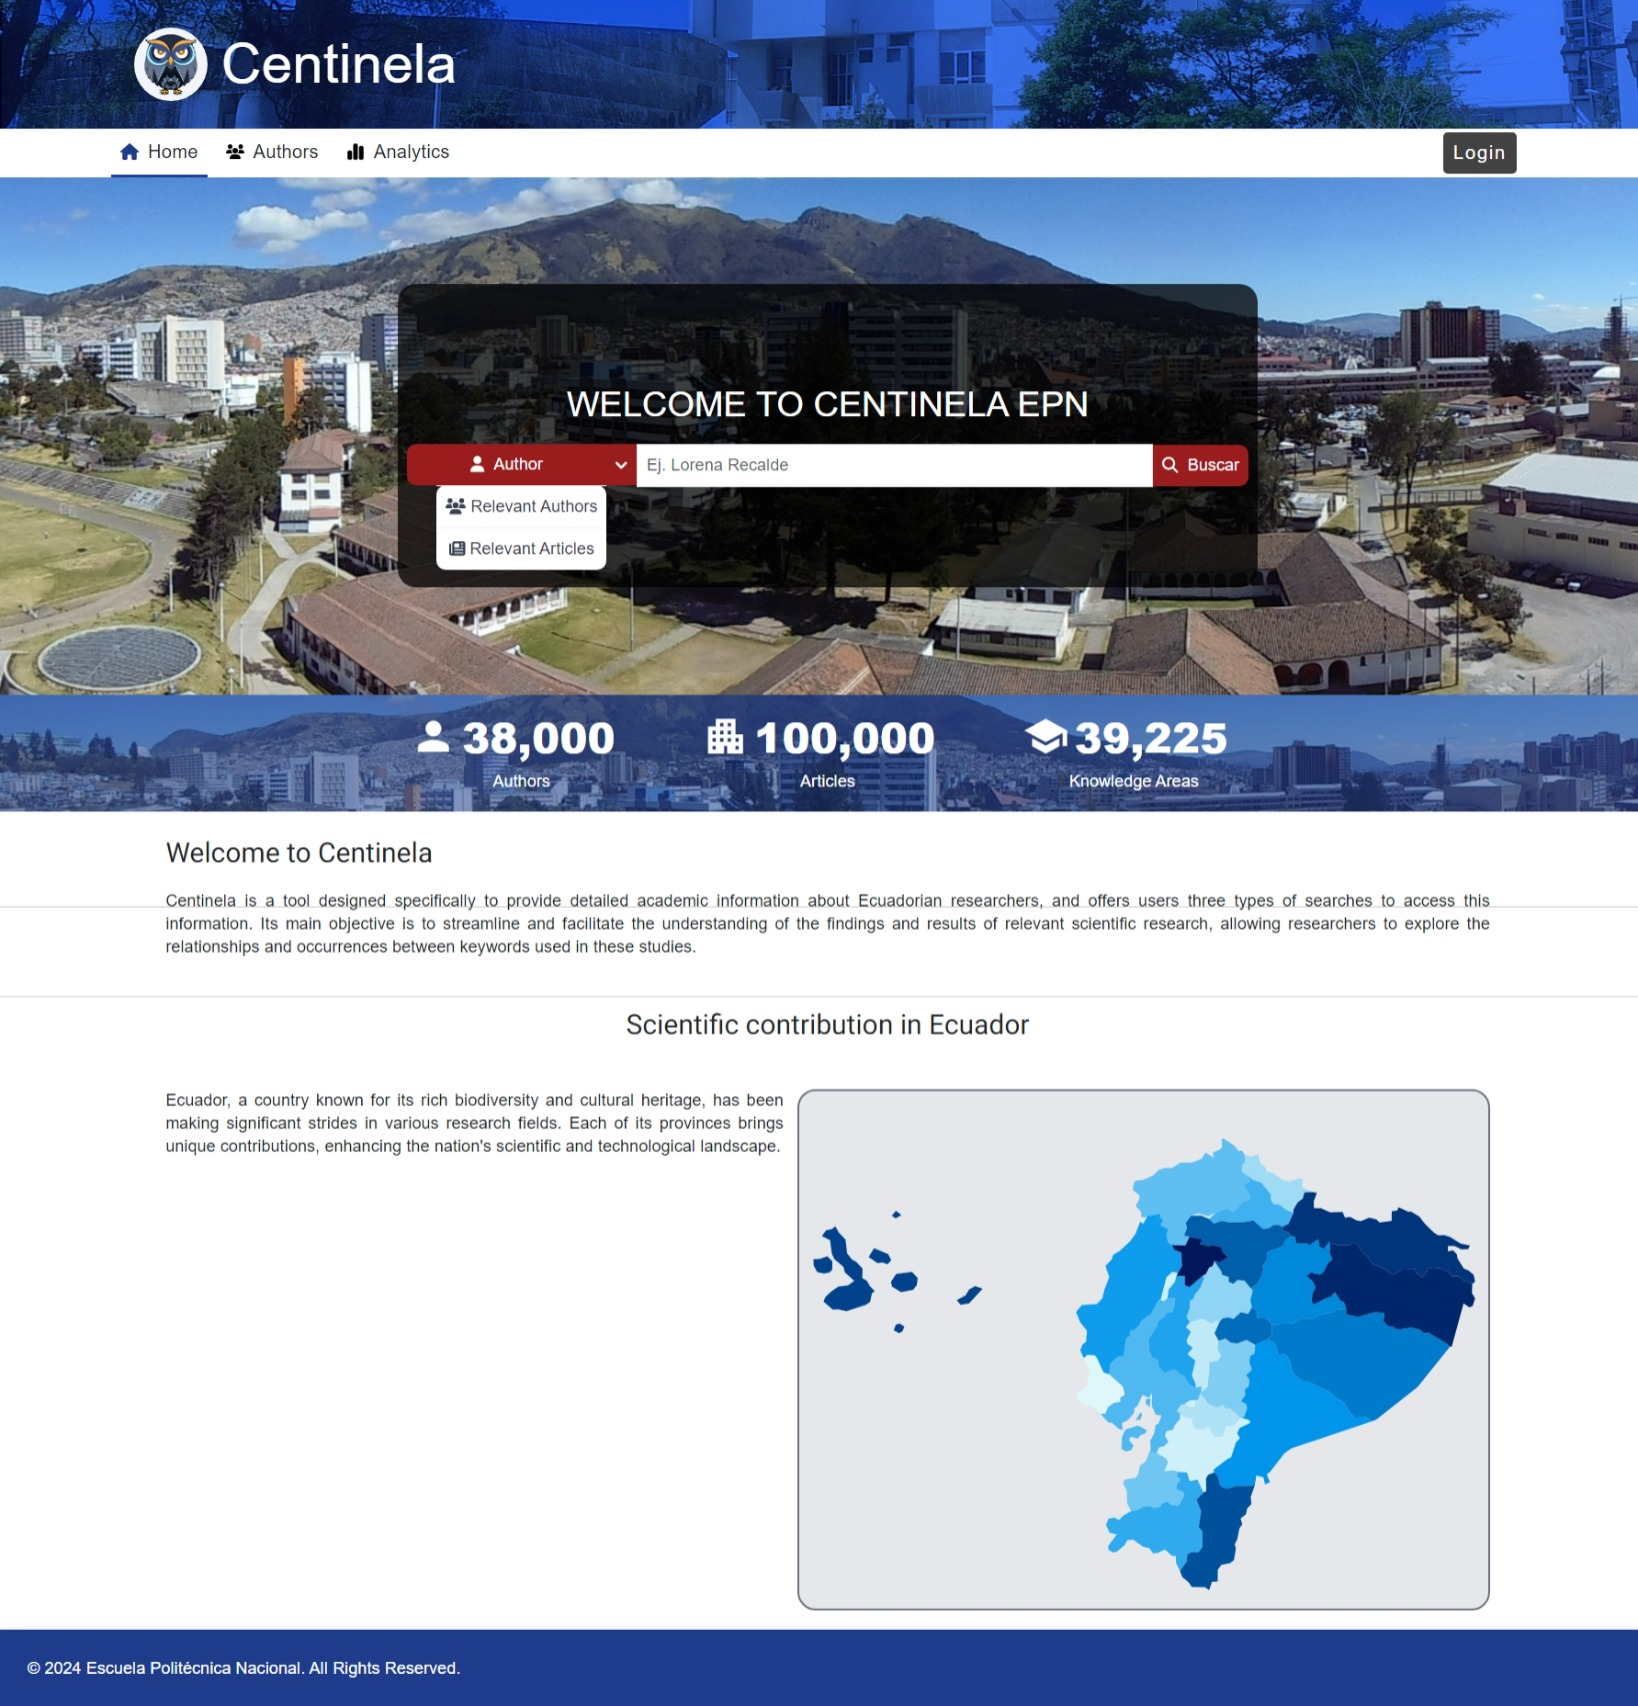
\includegraphics[scale=0.160]{../02Figures/02Chapter/Sprints/Sprint-1/home-page.jpeg}
    \caption{Página de inicio}
    \label{fig:home-page}
\end{figure}

\subsubsection{Página de resultados}
La página de resultados es la pantalla que se mostrará al usuario después de realizar una búsqueda en la aplicación.
En esta pantalla, se mostrarán los resultados de la búsqueda, que incluirán una lista de autores y artículos relevantes, dependiendo del tipo de búsqueda que haya realizado el usuario.
La figura \ref{fig:mockup-results} muestra el diseño de la página de resultados. Cabe destacar que esta página va a ser dinámica, es decir se modificará en función de los resultados de la búsqueda.
También contiene el componente de paginación, que permitirá al usuario navegar entre los resultados de la búsqueda. Este último está disponible para el tipo de búsqueda de autores por palabra clave y para el tipo de búsqueda de artículos relevantes por tópico, ya que estos tipos de búsqueda pueden devolver un gran número de resultados. Y al ser una aplicación web, se ha optado por mostrar 10 resultados por página para garantizar una buena experiencia de usuario y reducir tiempos de carga.

\begin{figure}[H]
    \centering
    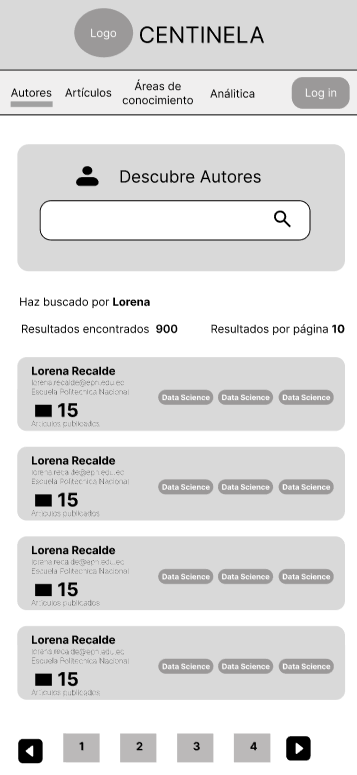
\includegraphics[scale=0.6]{../02Figures/02Chapter/Sprints/Sprint-1/mobile-first-results.png}
    \caption{Mockup de la página de resultados}
    \label{fig:mockup-results}
\end{figure}

Como se menciono en la Tabla \ref{fig:aceptance-criteria-HU-SE-01} y \ref{fig:aceptance-criteria-HU-SE-02} los criterios de aceptación de las historias de usuario HU-SE-01 y HU-SE-02 cada resultado tendrá que ser redirigido a una pantalla en donde 
se visualizará la información detallada del autor o del articulo. Para este caso en especifico se muestra el diseño para la pagina que tendrá
la información detallada de un autor, en la figura \ref{fig:mockup-article-detail}.
\begin{figure}[H]
    \centering
    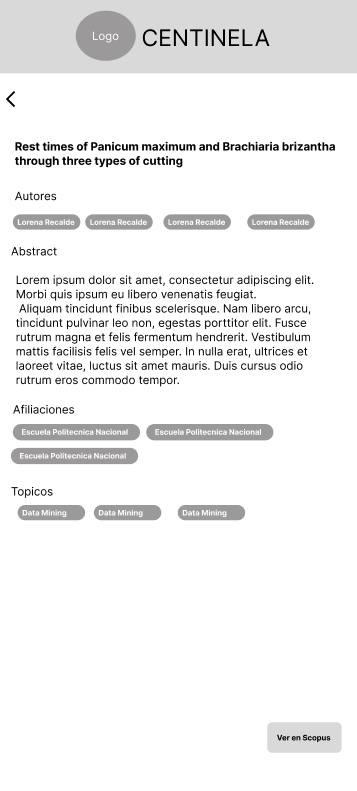
\includegraphics[scale=0.8]{../02Figures/02Chapter/Sprints/Sprint-1/article-detail.png}
    \caption{Mockup de la página de detalle del articulo}
    \label{fig:mockup-article-detail}
\end{figure}

Para el enrutamiento de la aplicación se ha utilizado el modulo de enrutamiento de Angular, el cual nos permite definir las rutas de la aplicación y asociarlas con los componentes correspondientes.
En la Figura \ref{fig:enrutamiento-article-page} se muestra el enrutamiento hacia el componente que contendrá la información general de un articulo. El mismo que como parámetro recibirá el id del articulo que se desea visualizar.
\begin{figure}[H]
    \centering
    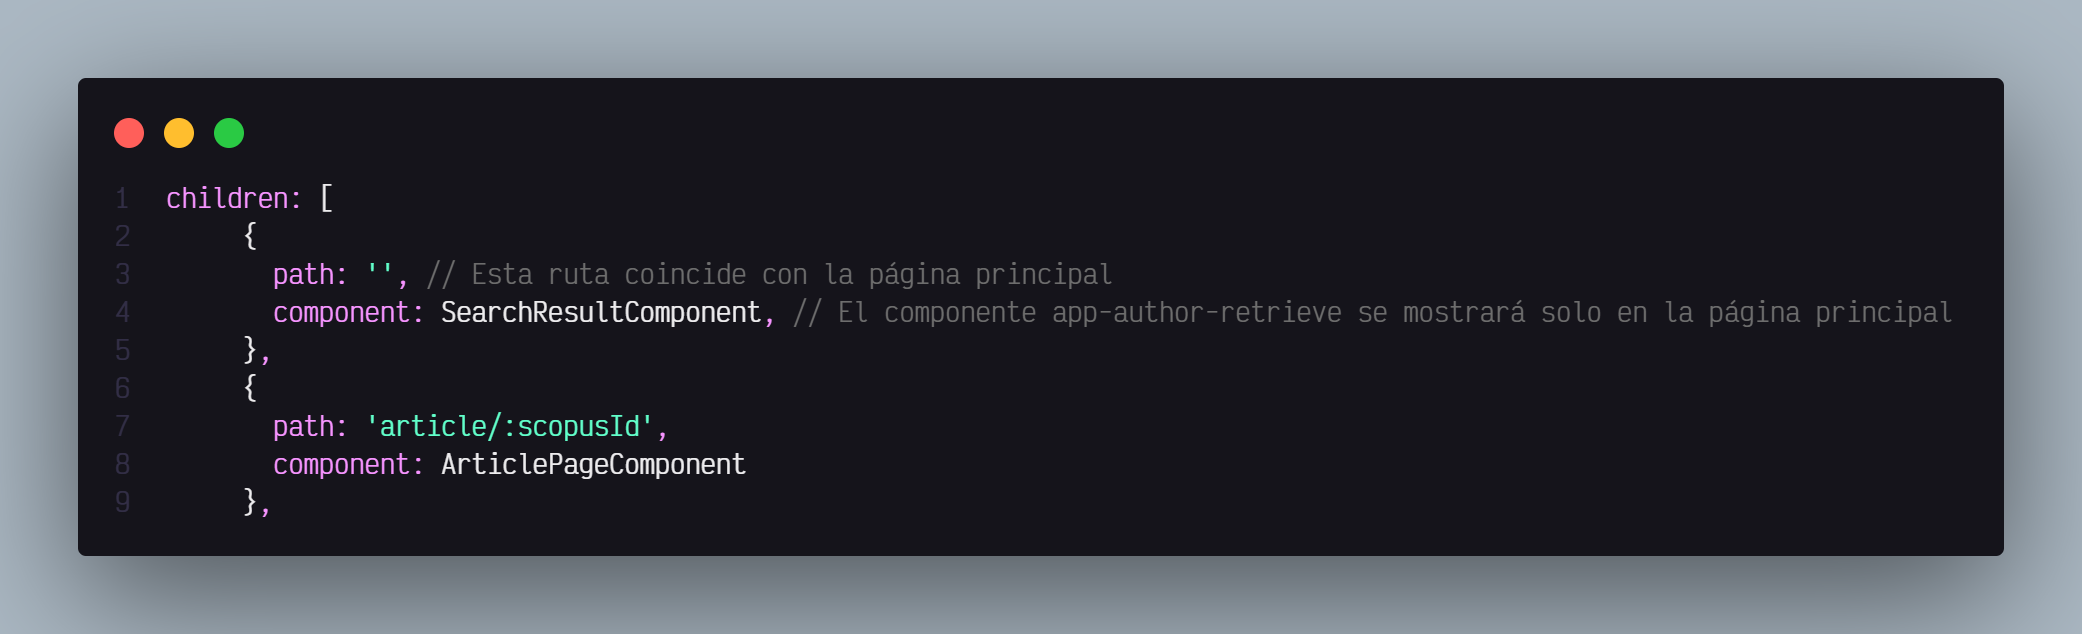
\includegraphics[scale=0.2]{../02Figures/02Chapter/Sprints/Sprint-1/enrutamiento-article-page.png}
    \caption{Routing de la página de detalle de articulo}
    \label{fig:enrutamiento-article-page}
\end{figure}

%% Aqui deseo mostrar ya la implementacion de la pagina de articulo pero da una descripcion de la misma
Resultado de la implementación de la página de información general de un articulo se muestra en la figura \ref{fig:article-page}.
En la que se muestra la información general de un articulo, como el titulo, resumen, autores, afiliaciones, palabras clave y el año de publicación. Asi como tambien un boton que permitira al usuario acceder al articulo completo en la pagina de Scopus.

\begin{figure}[H]
    \centering
    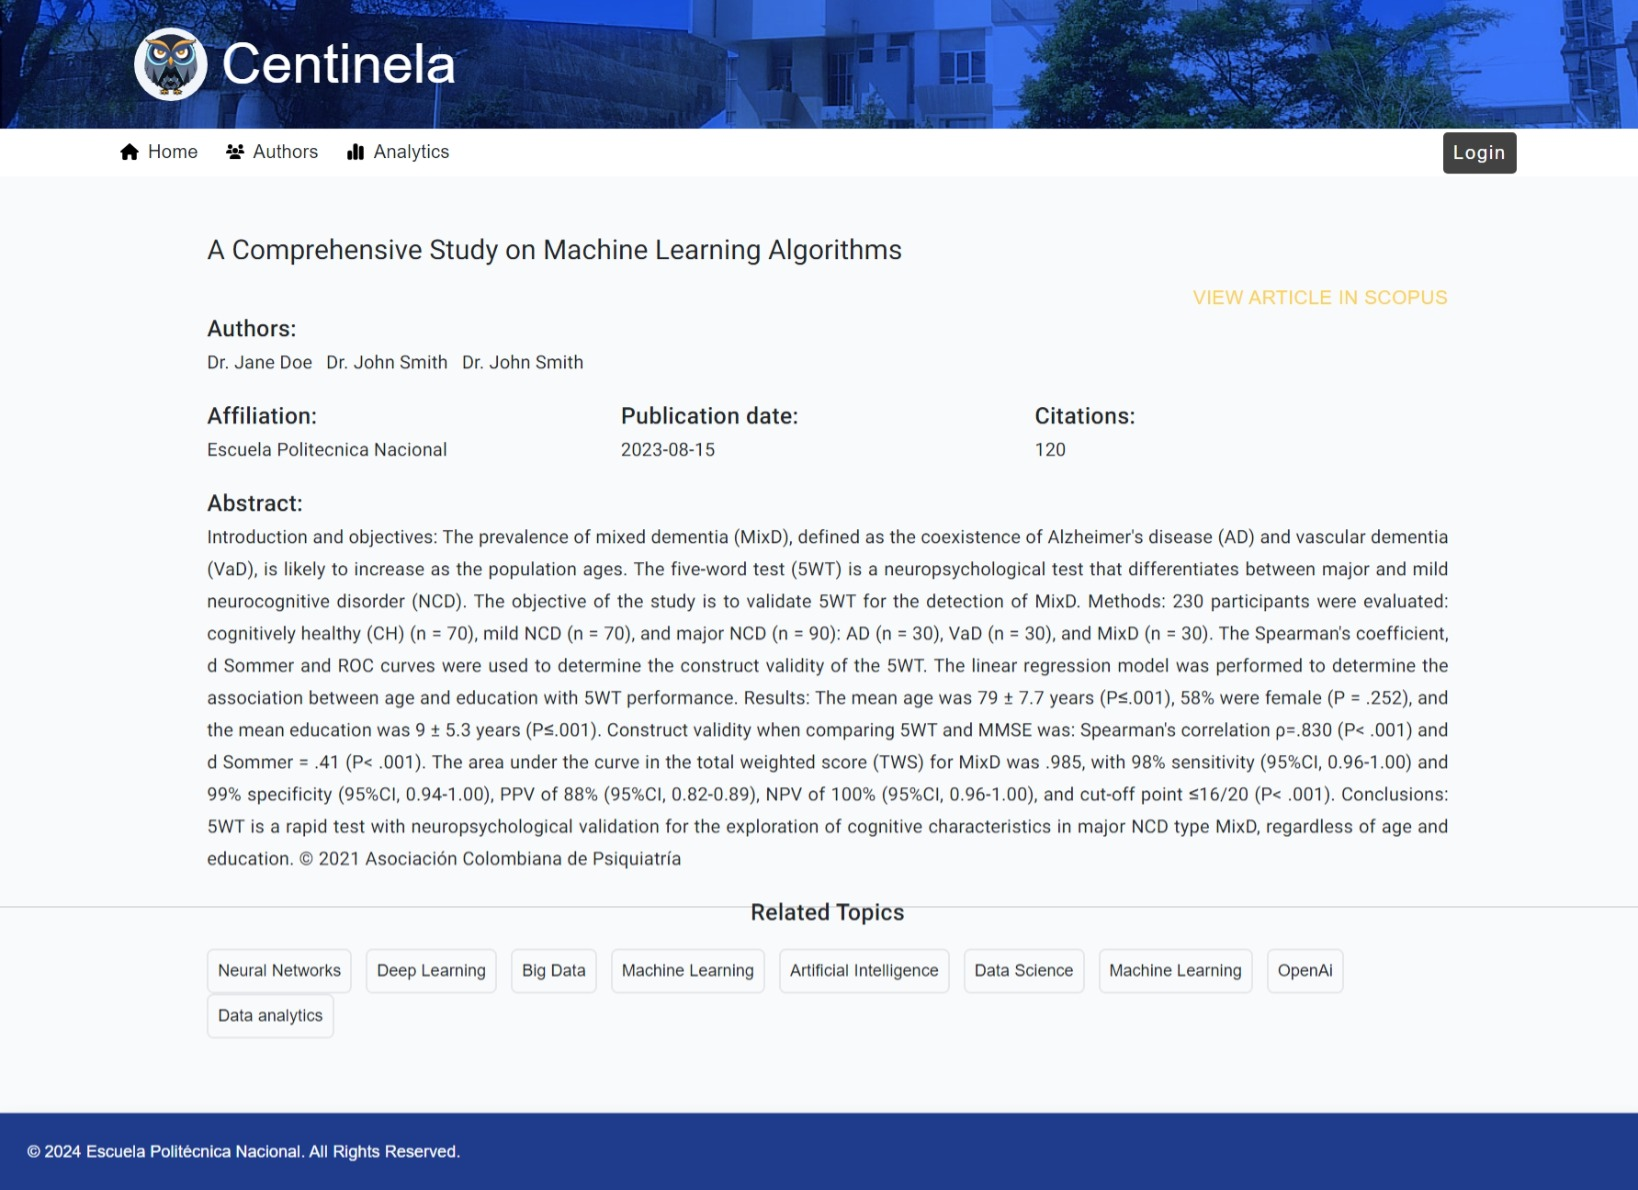
\includegraphics[scale=0.160]{../02Figures/02Chapter/Sprints/Sprint-1/article-page.jpeg}
    \caption{Página de detalle de articulo}
    \label{fig:article-page}
\end{figure}

%% Revision y Retrospectiva del sprint
\subsection{Revisión y Retrospectiva}
Durante este sprint, hemos logrado completar todas las historias de usuario planificadas, lo que nos ha permitido avanzar significativamente en el desarrollo de la aplicación.
Hemos creado los mockups de las interfaces de usuario de la aplicación, desarrollado la estructura principal del motor de búsqueda, implementado el enrutamiento de la aplicación y la página de inicio.
Además, hemos implementado la página de resultados y la página de información general de un artículo.
En general, el equipo ha trabajado de manera eficiente y colaborativa, lo que ha permitido cumplir con los objetivos del sprint en el tiempo previsto.
Sin embargo, hemos identificado algunas áreas de mejora que podrían ayudarnos a optimizar nuestro trabajo en futuros sprints.
\begin{itemize}
    \item \textbf{Comunicación}: Aunque hemos mantenido una comunicación constante a través de reuniones diarias y canales de mensajería, es importante mejorar la comunicación entre los miembros del equipo para garantizar que todos estén al tanto de los avances del proyecto.
    \item \textbf{Planificación}: Aunque hemos logrado completar todas las historias de usuario planificadas, es importante revisar y ajustar nuestra planificación para futuros sprints, teniendo en cuenta la complejidad y el tiempo requerido para cada tarea.
    \item \textbf{Colaboración}: Hemos trabajado de manera colaborativa y eficiente durante este sprint, lo que ha permitido cumplir con los objetivos del proyecto. Es importante seguir fomentando la colaboración entre los miembros del equipo para garantizar el éxito del proyecto.
    \item \textbf{Retroalimentación}: Es importante recopilar y analizar la retroalimentación de los usuarios para identificar áreas de mejora y realizar ajustes en futuras iteraciones del proyecto.
\end{itemize}

Cabe destacar que las tareas referentes a la integración de la aplicación con la API de Scopus, así como la implementación de funcionalidades del lado del servidor,
se han dejado para futuros sprints, ya que requieren un mayor tiempo de desarrollo y dependen de la finalización de otras tareas.


\section{Sprint 2}
\label{chapter02-section02-sprint2}

\subsection{Introducción}
Durante el segundo sprint se continuó con el desarrollo de la integración 
de las aplicaciones mencionadas en el sprint anterior.
Para este sprint en especifico se trabajó en los detalles sobre los autores, 
asi como su red de coautoría, articulos publicados y topicos de interes.

\subsection{Objetivos}
\begin{itemize}
    \item Implementar las ventanas para cada uno de los detalles de los autores.
    \item Integrar la fuerza de colaboración entre autores.
    \item Desarrollar la funcionalidad de articulos publicados por autor.
    \item Enrutamiento para las diferentes vistas de los autores.
\end{itemize}

\subsection{Planificación}
Para este sprint se selecciono un total de 2 historias de usuario, divididas en un total de
12 tareas a realizar las cuales fueron asignadas a los integrantes del equipo de desarrollo.

En la Tabla \ref{C2T2:Historias de Usuario del Sprint 2} se detallan las historias de usuario seleccionadas para este sprint.

\begin{table}[H]
    \centering
    \begin{tabular}{|p{2.5cm}|p{5cm}|p{6cm}|}
        \midrule
        \textbf{Identificador} & \textbf{Historia de Usuario}                                                                                                                                                                               & \textbf{Tareas} \\
        \hline
        HU-SE-03 & Como usuario no registrado, deseo poder ver la red de coautoría de un autor para visualizar un grafo con los autores con los que ha colaborado, así como la fuerza de esas colaboraciones &
        \begin{compactitem}
            \item Diseñar e implementar la interfaz y el grafo interactivo
            \item Definir y aplicar un esquema visual para la fuerza de la colaboración
            \item Implementar funcionalidades interactivas y filtros
            \item Agregar un panel de detalles con información adicional sobre el autor
        \end{compactitem}
        \\
        \hline
        HU-SE-04 & Como usuario no registrado quiero poder ver los artículos de un investigador para conocer su trabajo y las publicaciones en las que ha contribuido &
        \begin{compactitem}
            \item Diseñar la interfaz y enrutamiento para la lista de artículos
            \item Implementar la tabla de artículos y la funcionalidad de redirección
        \end{compactitem}
        \\
        \hline
        
    \end{tabular}
    \caption{Historias de Usuario del sprint 2}
    \label{C2T2:Historias de Usuario del Sprint 2}
\end{table}


Al igual que en el sprint anterior, cada historia de usuario se dividió en tareas más pequeñas,
las cuales se asignaron a los integrantes del equipo de desarrollo. Asi también se definieron
los criterios de aceptación que se muestran en la Figura \ref{C2F2:Criterios de Aceptacion HU-SE-03} y en la Figura \ref{C2F2:Criterios de Aceptacion HU-SE-04}.
para cada una con el fin de asegurar la calidad del desarrollo y
que cada miembro del equipo tuviera claro lo que se esperaba de la tarea asignada.
%%Input the figure

\begin{figure}[H]
    \centering
    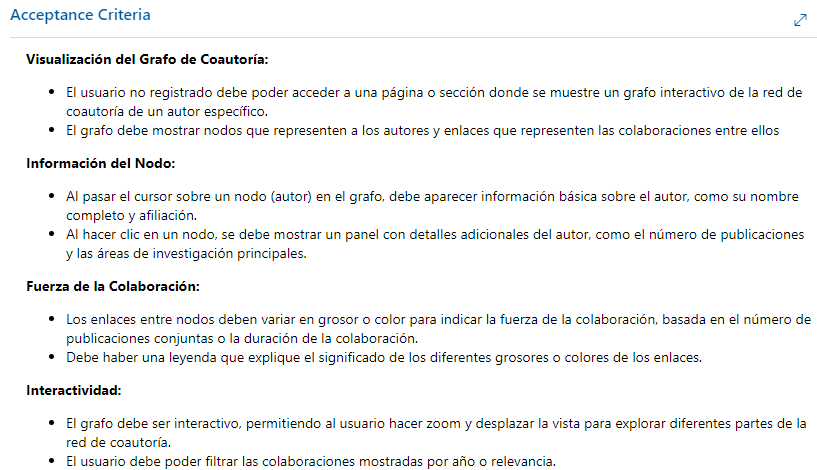
\includegraphics[width=0.8\textwidth]{../02Figures/02Chapter/Sprints/Sprint-2/aceptance-criteria-HU-SE-03.png}
    \caption{Criterios de Aceptación HU-SE-03}
    \label{C2F2:Criterios de Aceptacion HU-SE-03}
\end{figure}

\begin{figure}[H]
    \centering
    
\includegraphics[width=0.8\textwidth]{../02Figures/02Chapter/Sprints/Sprint-2/aceptance-criteria-HU-SE-04.png}
    \caption{Criterios de Aceptación HU-SE-04}
    \label{C2F2:Criterios de Aceptacion HU-SE-04}
\end{figure}

A continuación en la Figura \ref{fig:azure-board-sprint-2} se muestran las tareas de cada historia de usuario. Asi como en  Azure DevOps se crearon los \textit{work items} para cada tarea y se asignaron a los miembros del equipo.

\begin{figure}[H]
    \centering
    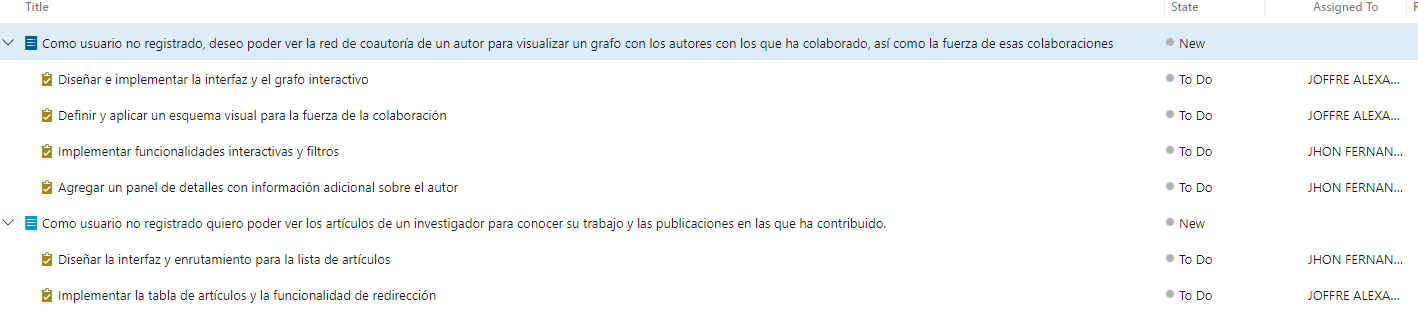
\includegraphics[width=1\textwidth]{../02Figures/02Chapter/Sprints/Sprint-2/fig_azure-board-sprint-2.png}
    \caption{Planificación de tareas del sprint 2}
    \label{fig:azure-board-sprint-2}
\end{figure}


\subsection{Implementación}
Al igual que el sprint anterior, se utilizó Figma para el diseño de los mockups de las vistas que posteriormente se implementarán utilizando Angular.
En la Figura \ref{fig:mobile-first-network} se muestra el diseño de la vista de los detalles de un autor. Así como los detalles que va tener su red de coautoría.

\begin{figure}[H]
    \centering
    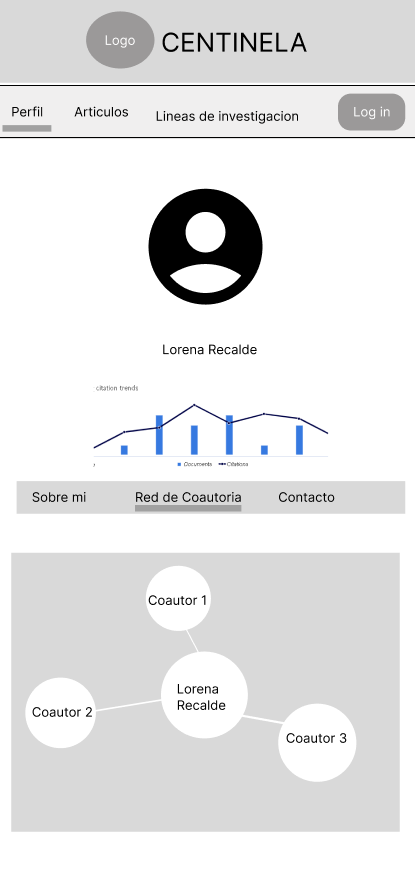
\includegraphics[scale=0.5]{../02Figures/02Chapter/Sprints/Sprint-2/mobile-first-network.png}
    \caption{Mockup de los detalles de un autor}
    \label{fig:mobile-first-network}
\end{figure}

Como se muestra en la Figura \ref{fig:mobile-first-network}, se diseñó la vista de los detalles de un autor, en la cual se muestra la red de coautoría del autor seleccionado. 
En la red de coautoría se muestra un grafo con los autores con los que ha colaborado, la fuerza de colaboración con cada autor se refleja en el grosor de la línea que los une.

En la Figura \ref{fig:mobile-first-articles} se muestra el diseño de la vista de los artículos publicados por un autor.
Los mismos estan representados en una tabla con la información de cada uno y contendran la interactividad que permitira al usuario redirigir al mockup de la Figura \ref{fig:mockup-article-detail}.

\begin{figure}[H]
    \centering
    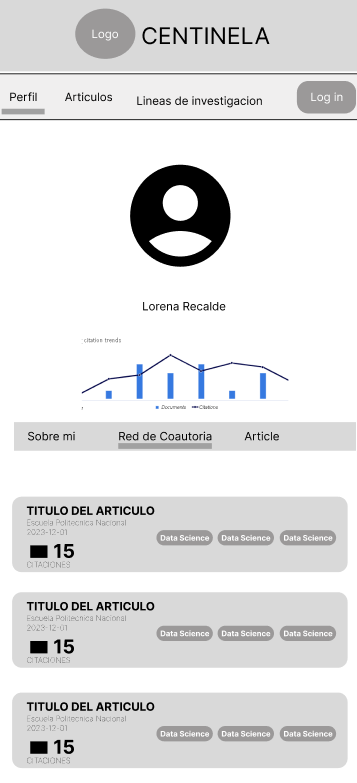
\includegraphics[scale=0.5]{../02Figures/02Chapter/Sprints/Sprint-2/mobile-first-articles.png}
    \caption{Mockup de los artículos publicados por un autor}
    \label{fig:mobile-first-articles}
\end{figure}

Para implementar la red de Coautoría se utilizó la librería D3.js, la cual permite la creación de gráficos interactivos en la web.
Para ello primero debemos definir los nodos y las relaciones entre ellos, en este caso los autores y la fuerza de colaboración entre ellos.
En la Figura \ref{fig:network-interface-ts} se muestra la interfaz en Typescript que servira para la creación de la red de coautoría.

\begin{figure}[H]
    \centering
    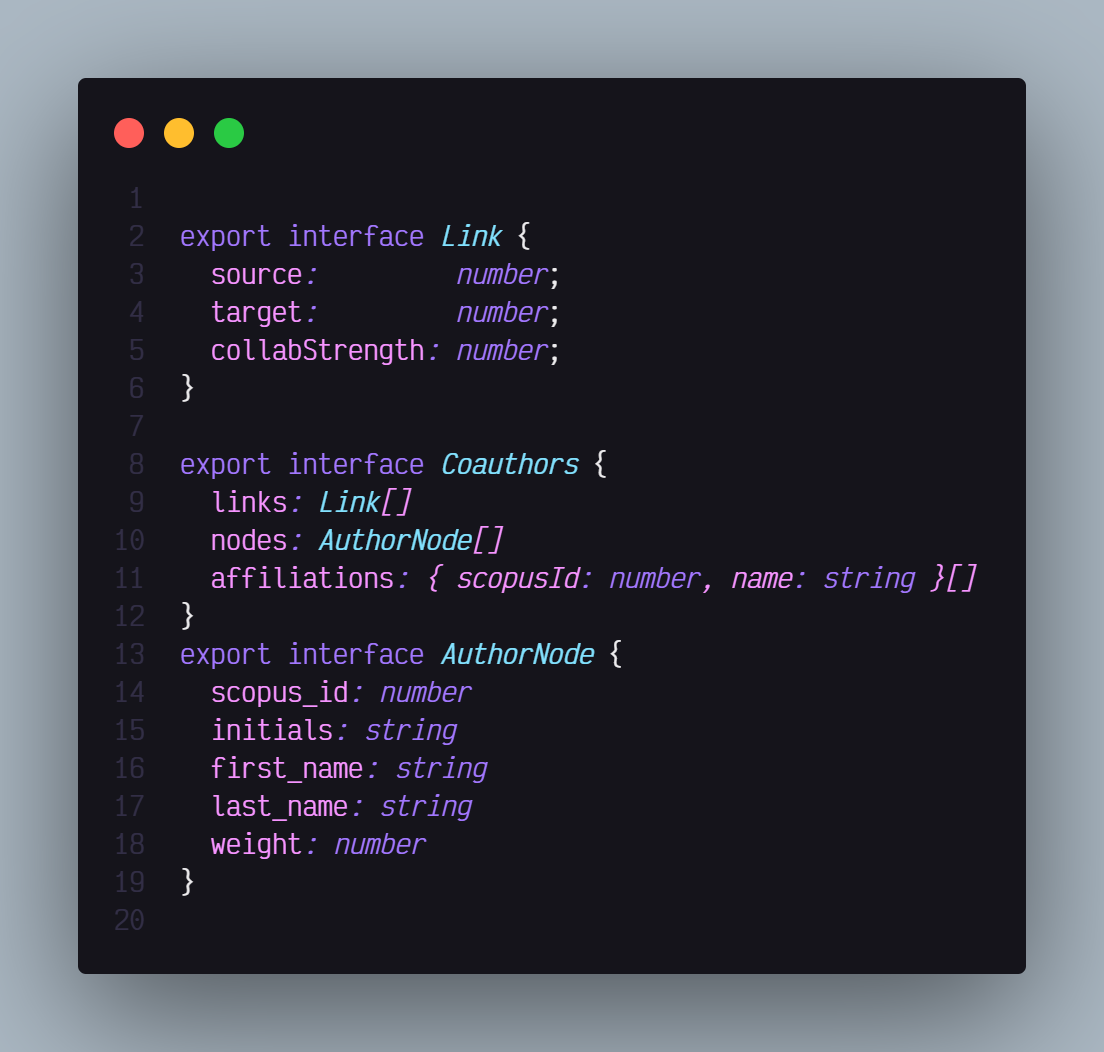
\includegraphics[scale=0.26]{../02Figures/02Chapter/Sprints/Sprint-2/coauthors-interface-typescript.png}
    \caption{Interfaz en Typescript para la creación de la red de coautoría}
    \label{fig:network-interface-ts}
\end{figure}

Debido a que el actual componente no se encargara de la creación de la red, sino que se encargará de la visualización de la misma. No se ahondará en la implementación de la red de coautoría, ya que se encuentra fuera del alcance de este documento.
El resultado final de la red de coautoría se muestra en la Figura \ref{fig:network-coauthors}.
\begin{figure}[H]
    \centering
    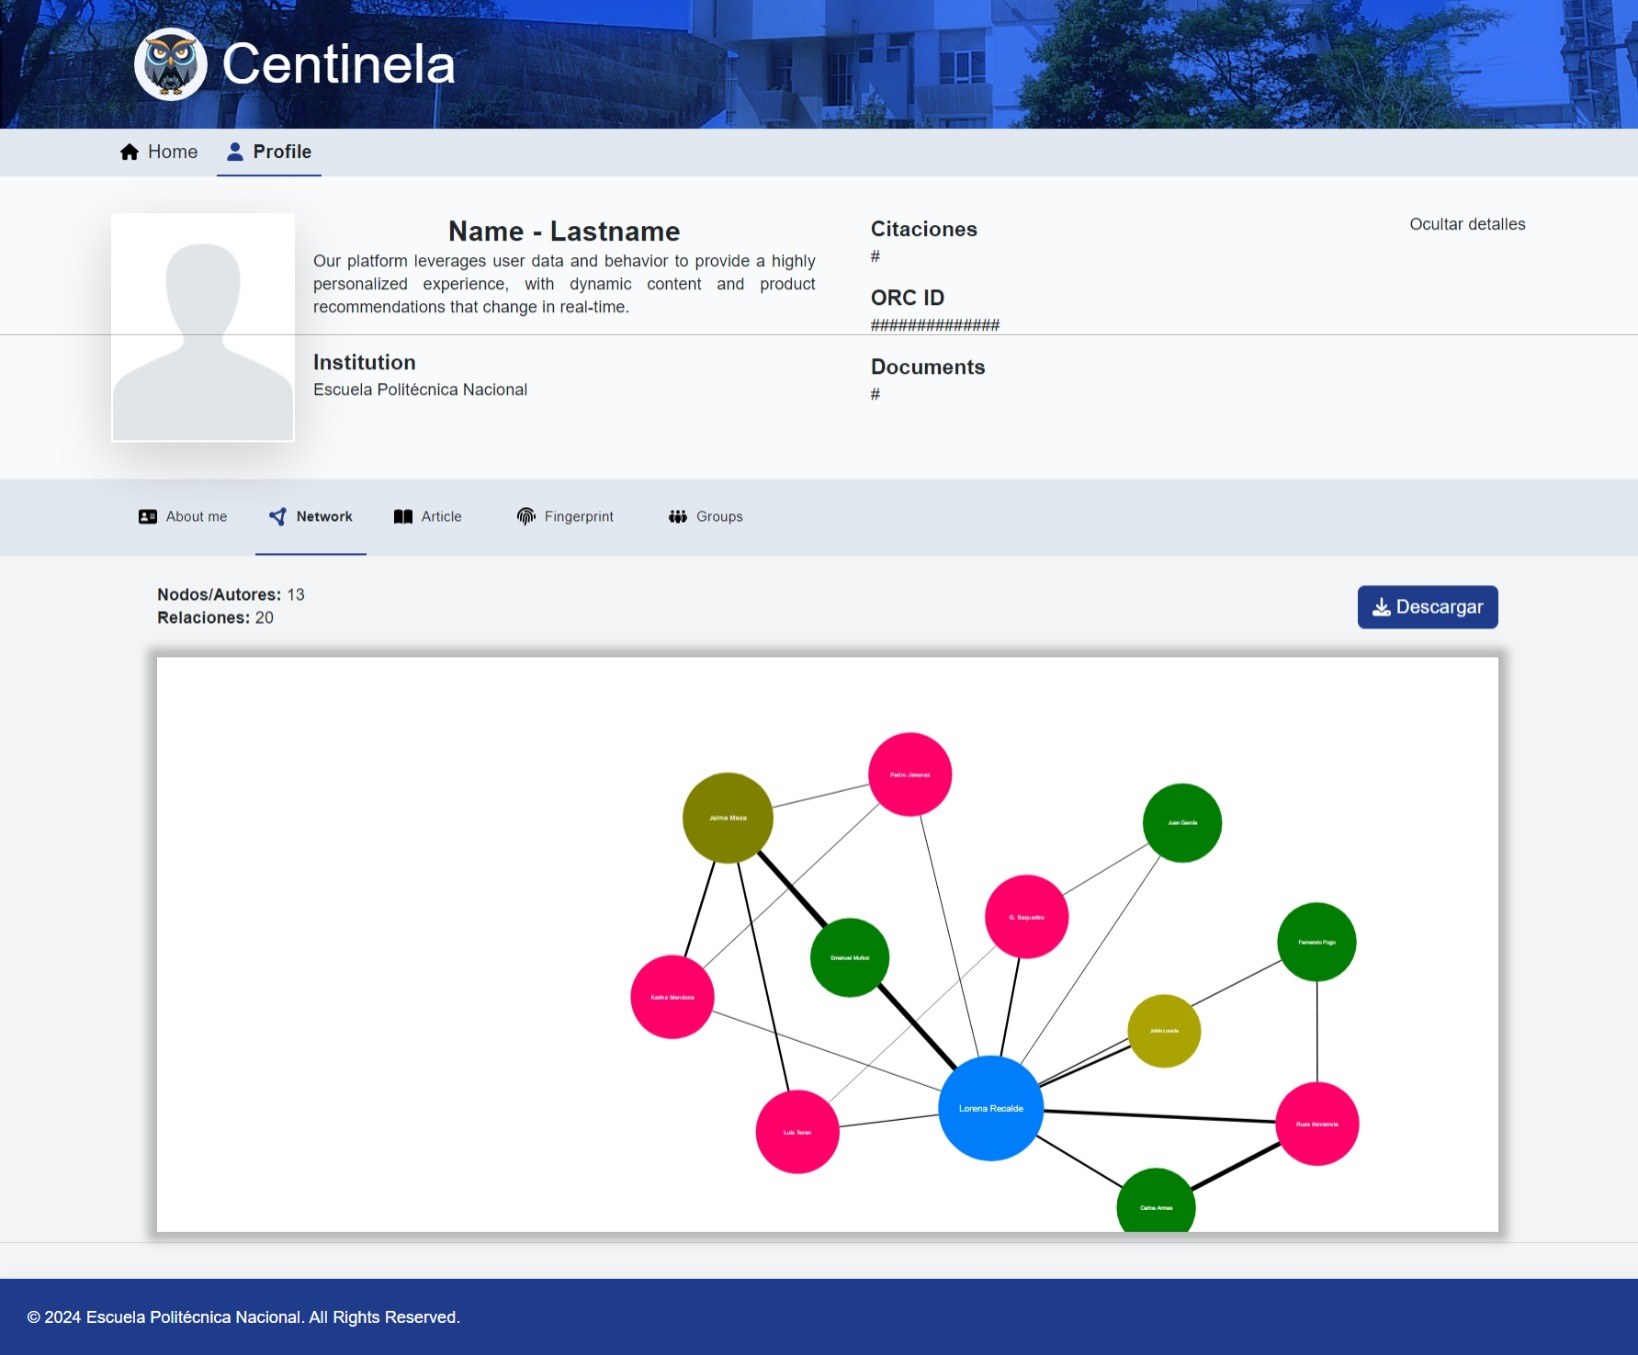
\includegraphics[scale=0.25]{../02Figures/02Chapter/Sprints/Sprint-2/network-coauthors.jpeg}
    \caption{Red de coautoría}
    \label{fig:network-coauthors}
\end{figure}

Cabe mencionar que para armar la red de coautoría que se muestra en la Figura \ref{fig:network-coauthors} se utilizó un conjunto de datos de prueba, ya que  de momento la aplicación no cuenta con la información necesaria para armar la red de coautoría.

Ahora en la Figura \ref{fig:articles-table} se muestra la tabla de los artículos publicados por un autor. Esta tabla también contendrá la interactividad que permitirá al usuario redirigir al mockup de la Figura \ref{fig:mockup-article-detail}.
\begin{figure}[H]
    \centering
    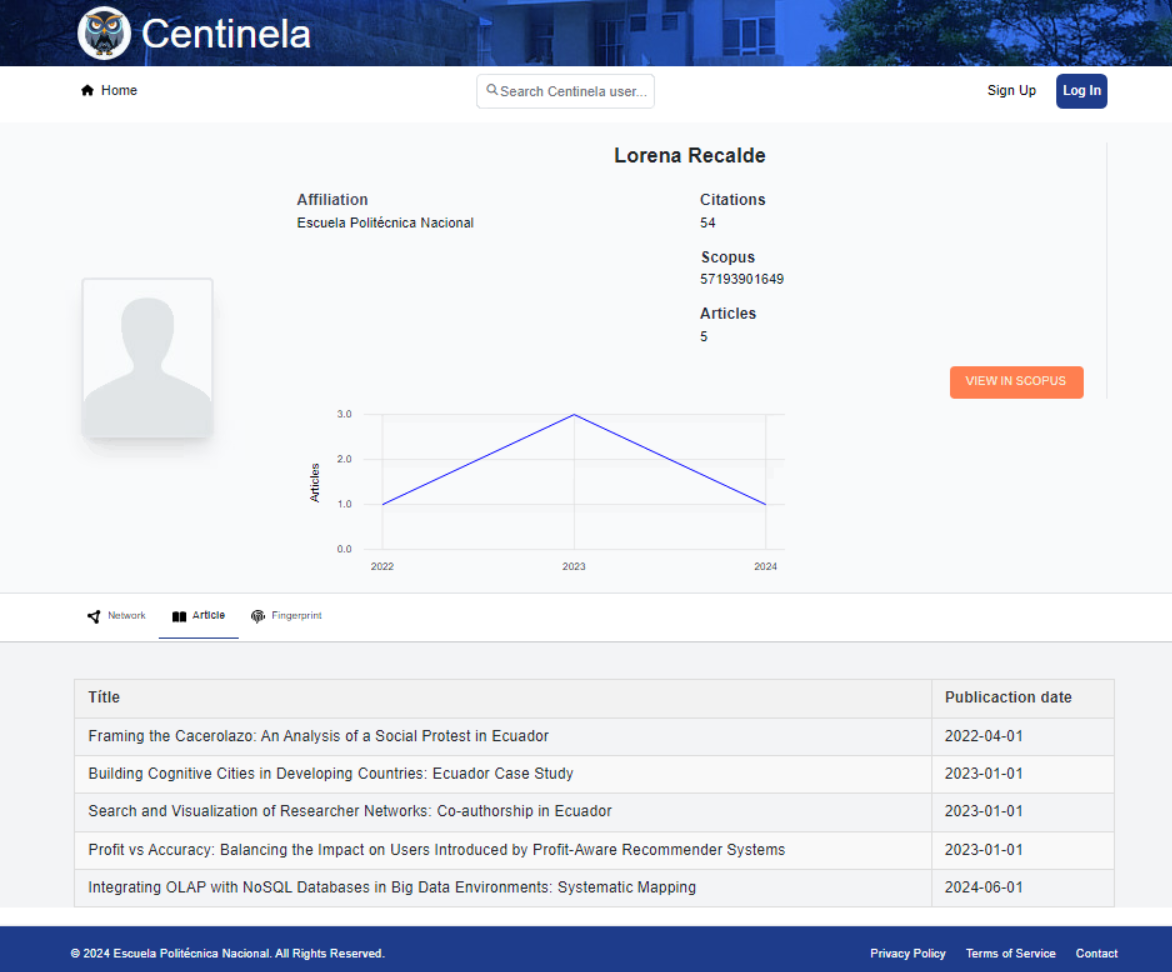
\includegraphics[scale=0.5]{../02Figures/02Chapter/Sprints/Sprint-2/article-table.png}
    \caption{Tabla de artículos publicados por un autor}
    \label{fig:articles-table}
\end{figure}

Para el despliegue de la aplicación en este sprint se utilizo Render como plataforma de despliegue, la cual permite el despliegue de aplicaciones web de forma gratuita.
En la Figura \ref{fig:render-deploy} se muestra el despliegue de la aplicación en Render.

%
%\begin{figure}[H]
%    \centering
%    \includegraphics[scale=0.5]{../02Figures/02Chapter/Sprints/Sprint-2/render-deploy.png}
%    \caption{Despliegue de la aplicación en Render}
%    \label{fig:render-deploy}
%\end{figure}

\subsection{Revisión y Retrospectiva}
Como resultado de este sprint se logró implementar las ventanas para cada uno de los detalles de los autores, la integración de la fuerza de colaboración entre autores, la funcionalidad de los artículos publicados por autor y el enrutamiento para las diferentes vistas de los autores.
Se logró cumplir con los objetivos planteados para este sprint, sin embargo, se presentaron algunos problemas durante el desarrollo de las tareas asignadas.
Uno de los problemas que se presentó fue la falta de información necesaria para la creación de la red de coautoría, ya que la aplicación no cuenta con la información necesaria para armar la red de coautoría.
Debido a que la implementación de la extracción de la información desde scopus se realizará en el siguiente sprint, sin embargo los servicios que se encargan de construir la red de coautoría ya se encuentran implementados y listos para recibir la información necesaria.

Al igual que en el Sprint anterior, las tareas relacionadas con la integración con Scopus quedaron pendientes, ya que se decidió que la implementación de la extracción de la información desde Scopus se realizará iniciara en el siguiente Sprint.


\section{Sprint 3}
\label{chapter02-section02-sprint3}
\subsection{Introducción}
\label{section:introduction-sprint-3}
A partir de este Sprint, se comenzará a implementar la integración con Scopus y toda lógica relacionada con el servidor. 

Para este Sprint específico, se establecerá el ambiente de desarrollo con las herramientas necesarias para la implementación.
Además, se rediseñará la base de datos orientada a grafos utilizando Neo4j, Django y Neomodel como ORM, basándonos en el diseño en Neo4j propuesto en Resnet.
Se trabajará en la implementación de los modelos en Neomodel.

Finalmente, se pretende exponer el uso de Arquitectura Hexagonal para la implementación de la funcionalidad de búsqueda de autores. Cabe destacar que este será el único sprint en el que se ahondará en la Arquitectura Hexagonal;
los demás sprints no tendrán ese nivel de detalle.

\subsection{Objetivos}

\begin{itemize}
    \item Levantar el ambiente de desarrollo
    \item Implementar y rediseñar los modelos de la base de datos en Neo4j a través de Neomodel.
    \item Desarrollar la funcionalidad de búsqueda de autores.
\end{itemize}

\subsection{Planificación}

Para este sprint se ha seleccionado las historias de usuario que se muestran en la tabla \ref{C2T3:Historias de Usuario del Sprint 3}.

\begin{table}[H]
    \centering
    \begin{tabular}{|p{2.5cm}|p{5cm}|p{6cm}|}
        \midrule
        \textbf{Identificador} & \textbf{Historia de Usuario}                                                                                                                                                                               & \textbf{Tareas} \\
        \hline
        HU-SE-02 & Como usuario no registrado deseo poder ver los investigadores que tengan colaboraciones en artículos con afiliaciones ecuatorianas para mantenerme informado sobre sus investigaciones y campos de estudio &
        \begin{compactitem}
            \item Crear servicios para el modelo de autor
            \item Diseñar el endpoint que maneje las solicitudes del autor
        \end{compactitem}
        \\
        \hline
        HU-SE-05 & Como desarrollador de software, quiero migrar nuestro modelo de base de datos actual a Neomodel, para que podamos aprovechar las capacidades del ORM Neomodel para simplificar la gestión de datos y mejorar la integración con nuestro proyecto Django.&
        \begin{compactitem}
            \item Definir los modelos, relaciones y propiedades de los nodos.
            \item Hacer las migraciones desde Django a Neo4j.
        \end{compactitem}
        \\
        \hline
        HU-SE-06 & Como desarrollador, quiero configurar un entorno de desarrollo replicable, para asegurar que podamos contar con un entorno completamente aislado y consistente que optimice el flujo de trabajo&
        \begin{compactitem}
            \item Crear el contenedor de Docker para al aplicación de backend
            \item Crear  un orquestador de contenedores
            \item Orquestar los servicios de la aplicación y la base de datos
        \end{compactitem}
        \\
        \hline
    \end{tabular}
    \caption{Historias de Usuario del sprint 3}
    \label{C2T3:Historias de Usuario del Sprint 3}
\end{table}


A continuación en las Figuras \ref{fig:aceptance-criteria-HU-SE-02}, \ref{fig:aceptance-criteria-HU-SE-05} y \ref{fig:aceptance-criteria-HU-SE-06}
se muestran los criterios de aceptación para las historias de usuario seleccionadas.
\begin{figure}[H]
    \centering
    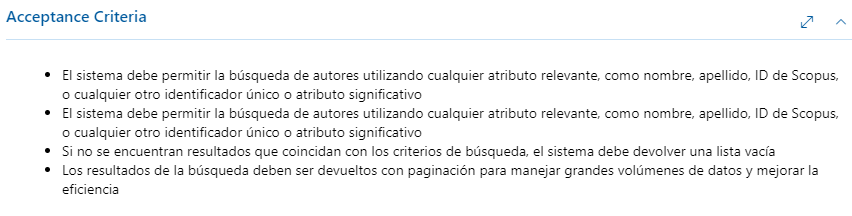
\includegraphics[scale=0.7]{../02Figures/02Chapter/Sprints/Sprint-3/aceptance-criteria-HU-SE-02.png}
    \caption{Criterios de aceptación HU-SE-02}
    \label{fig:aceptance-criteria-HU-SE-02}
\end{figure}

\begin{figure}[H]
    \centering
    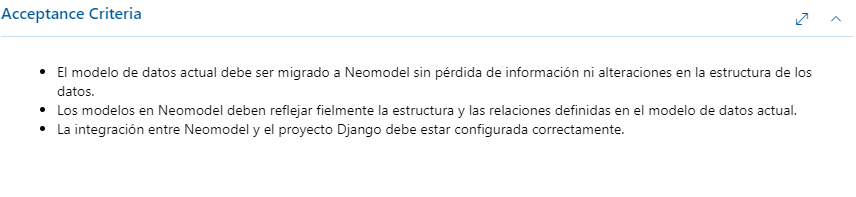
\includegraphics[scale=0.7]{../02Figures/02Chapter/Sprints/Sprint-3/aceptance-criteria-HU-SE-05.png}
    \caption{Criterios de aceptación HU-SE-05}
    \label{fig:aceptance-criteria-HU-SE-05}
\end{figure}

\begin{figure}[H]
    \centering
    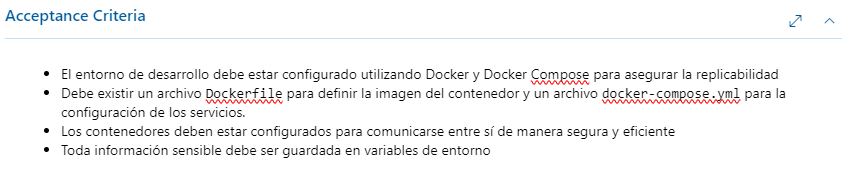
\includegraphics[scale=0.7]{../02Figures/02Chapter/Sprints/Sprint-3/aceptance-criteria-HU-SE-06.png}
    \caption{Criterios de aceptación HU-SE-06}
    \label{fig:aceptance-criteria-HU-SE-06}
\end{figure}

\subsection{Implementación}
Para el desarrollo del Sprint 3 se empezó con la configuración del entorno de desarrollo, se utilizó Docker para la creación de contenedores y Docker Compose para la orquestación de los servicios.
Para dockerizar la aplicación se creó un archivo Dockerfile en la raíz del proyecto, en el cual se especifican las instrucciones necesarias para la creación de la imagen de la aplicación, tal como se muestra Figura \ref{fig:dockerfile}.

\begin{figure}[!t]
    \centering
    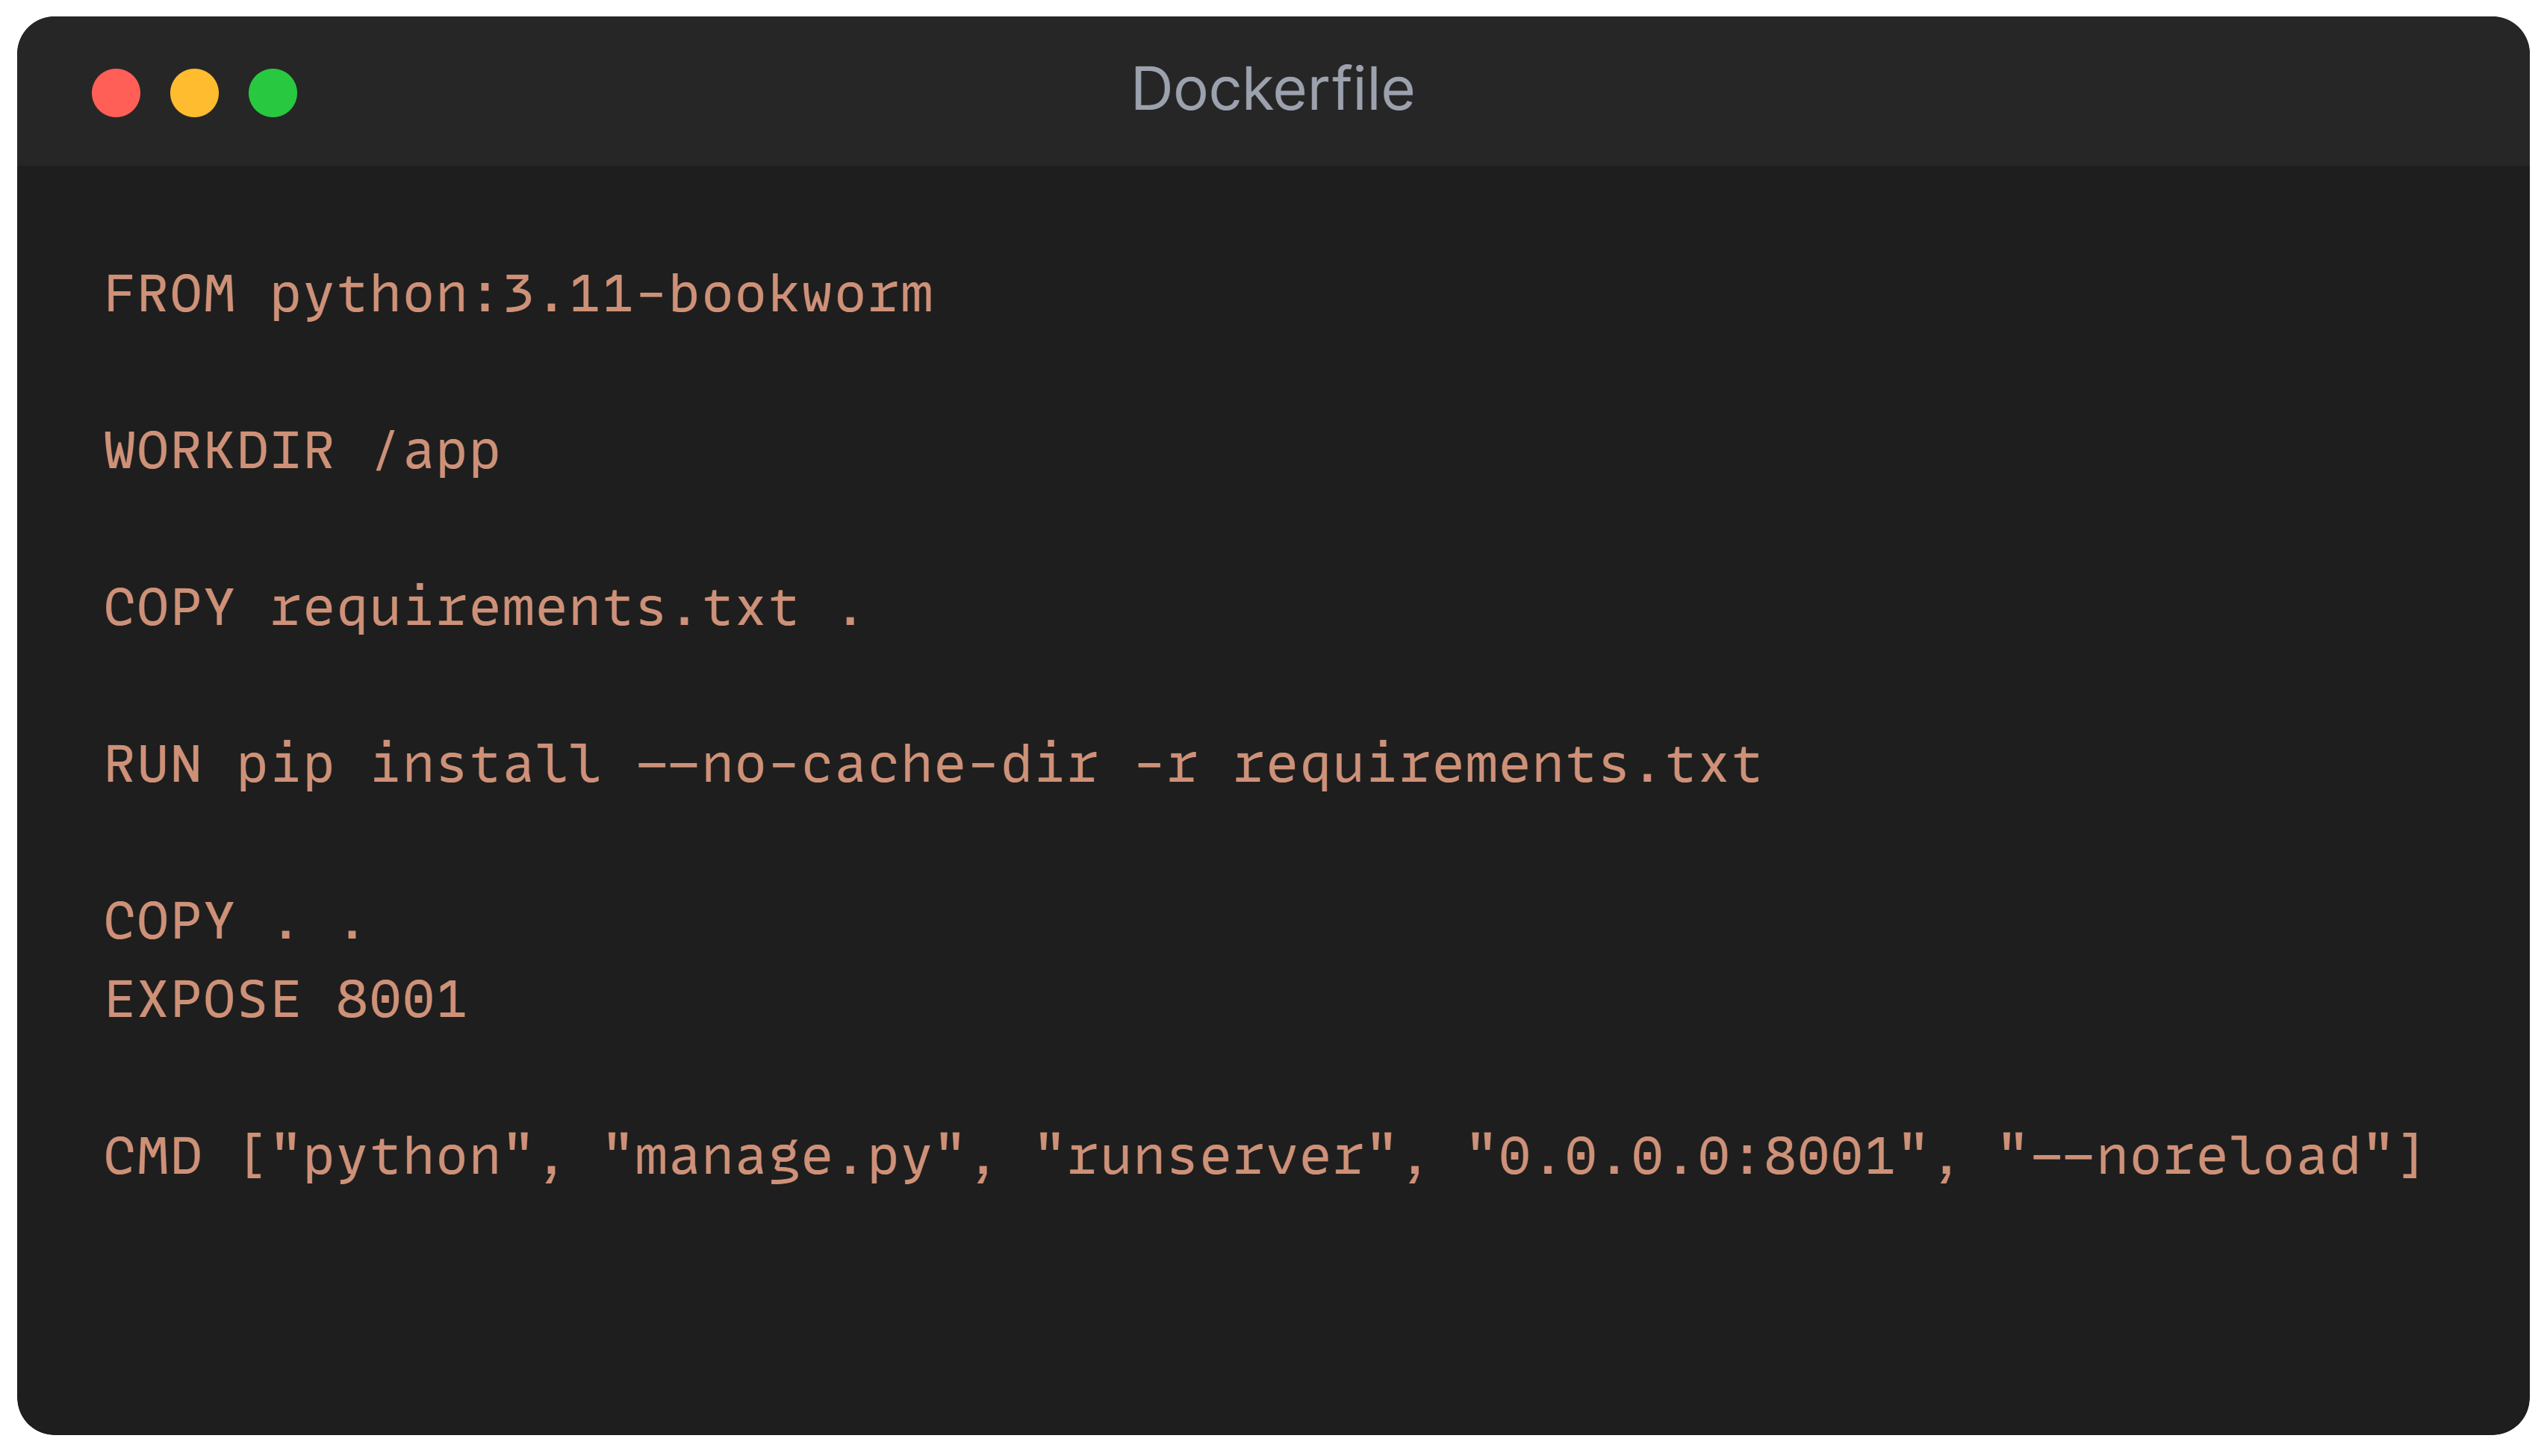
\includegraphics[scale=0.12]{../02Figures/02Chapter/Sprints/Sprint-3/Dockerfile.png}
    \caption{Archivo Dockerfile}
    \label{fig:dockerfile}
\end{figure}

En la Figura \ref{fig:docker-compose} se muestra el archivo de configuración de Docker Compose.
El mismo se encarga de orquestar los servicios de la aplicación y la base de datos. También se asegura de persistir los datos de la base de datos en un volumen de Docker.
De la misma manera se especifican las variables de entorno necesarias para la configuración y el correcto funcionamiento de la aplicación.

\begin{figure}[!t]
    \centering
    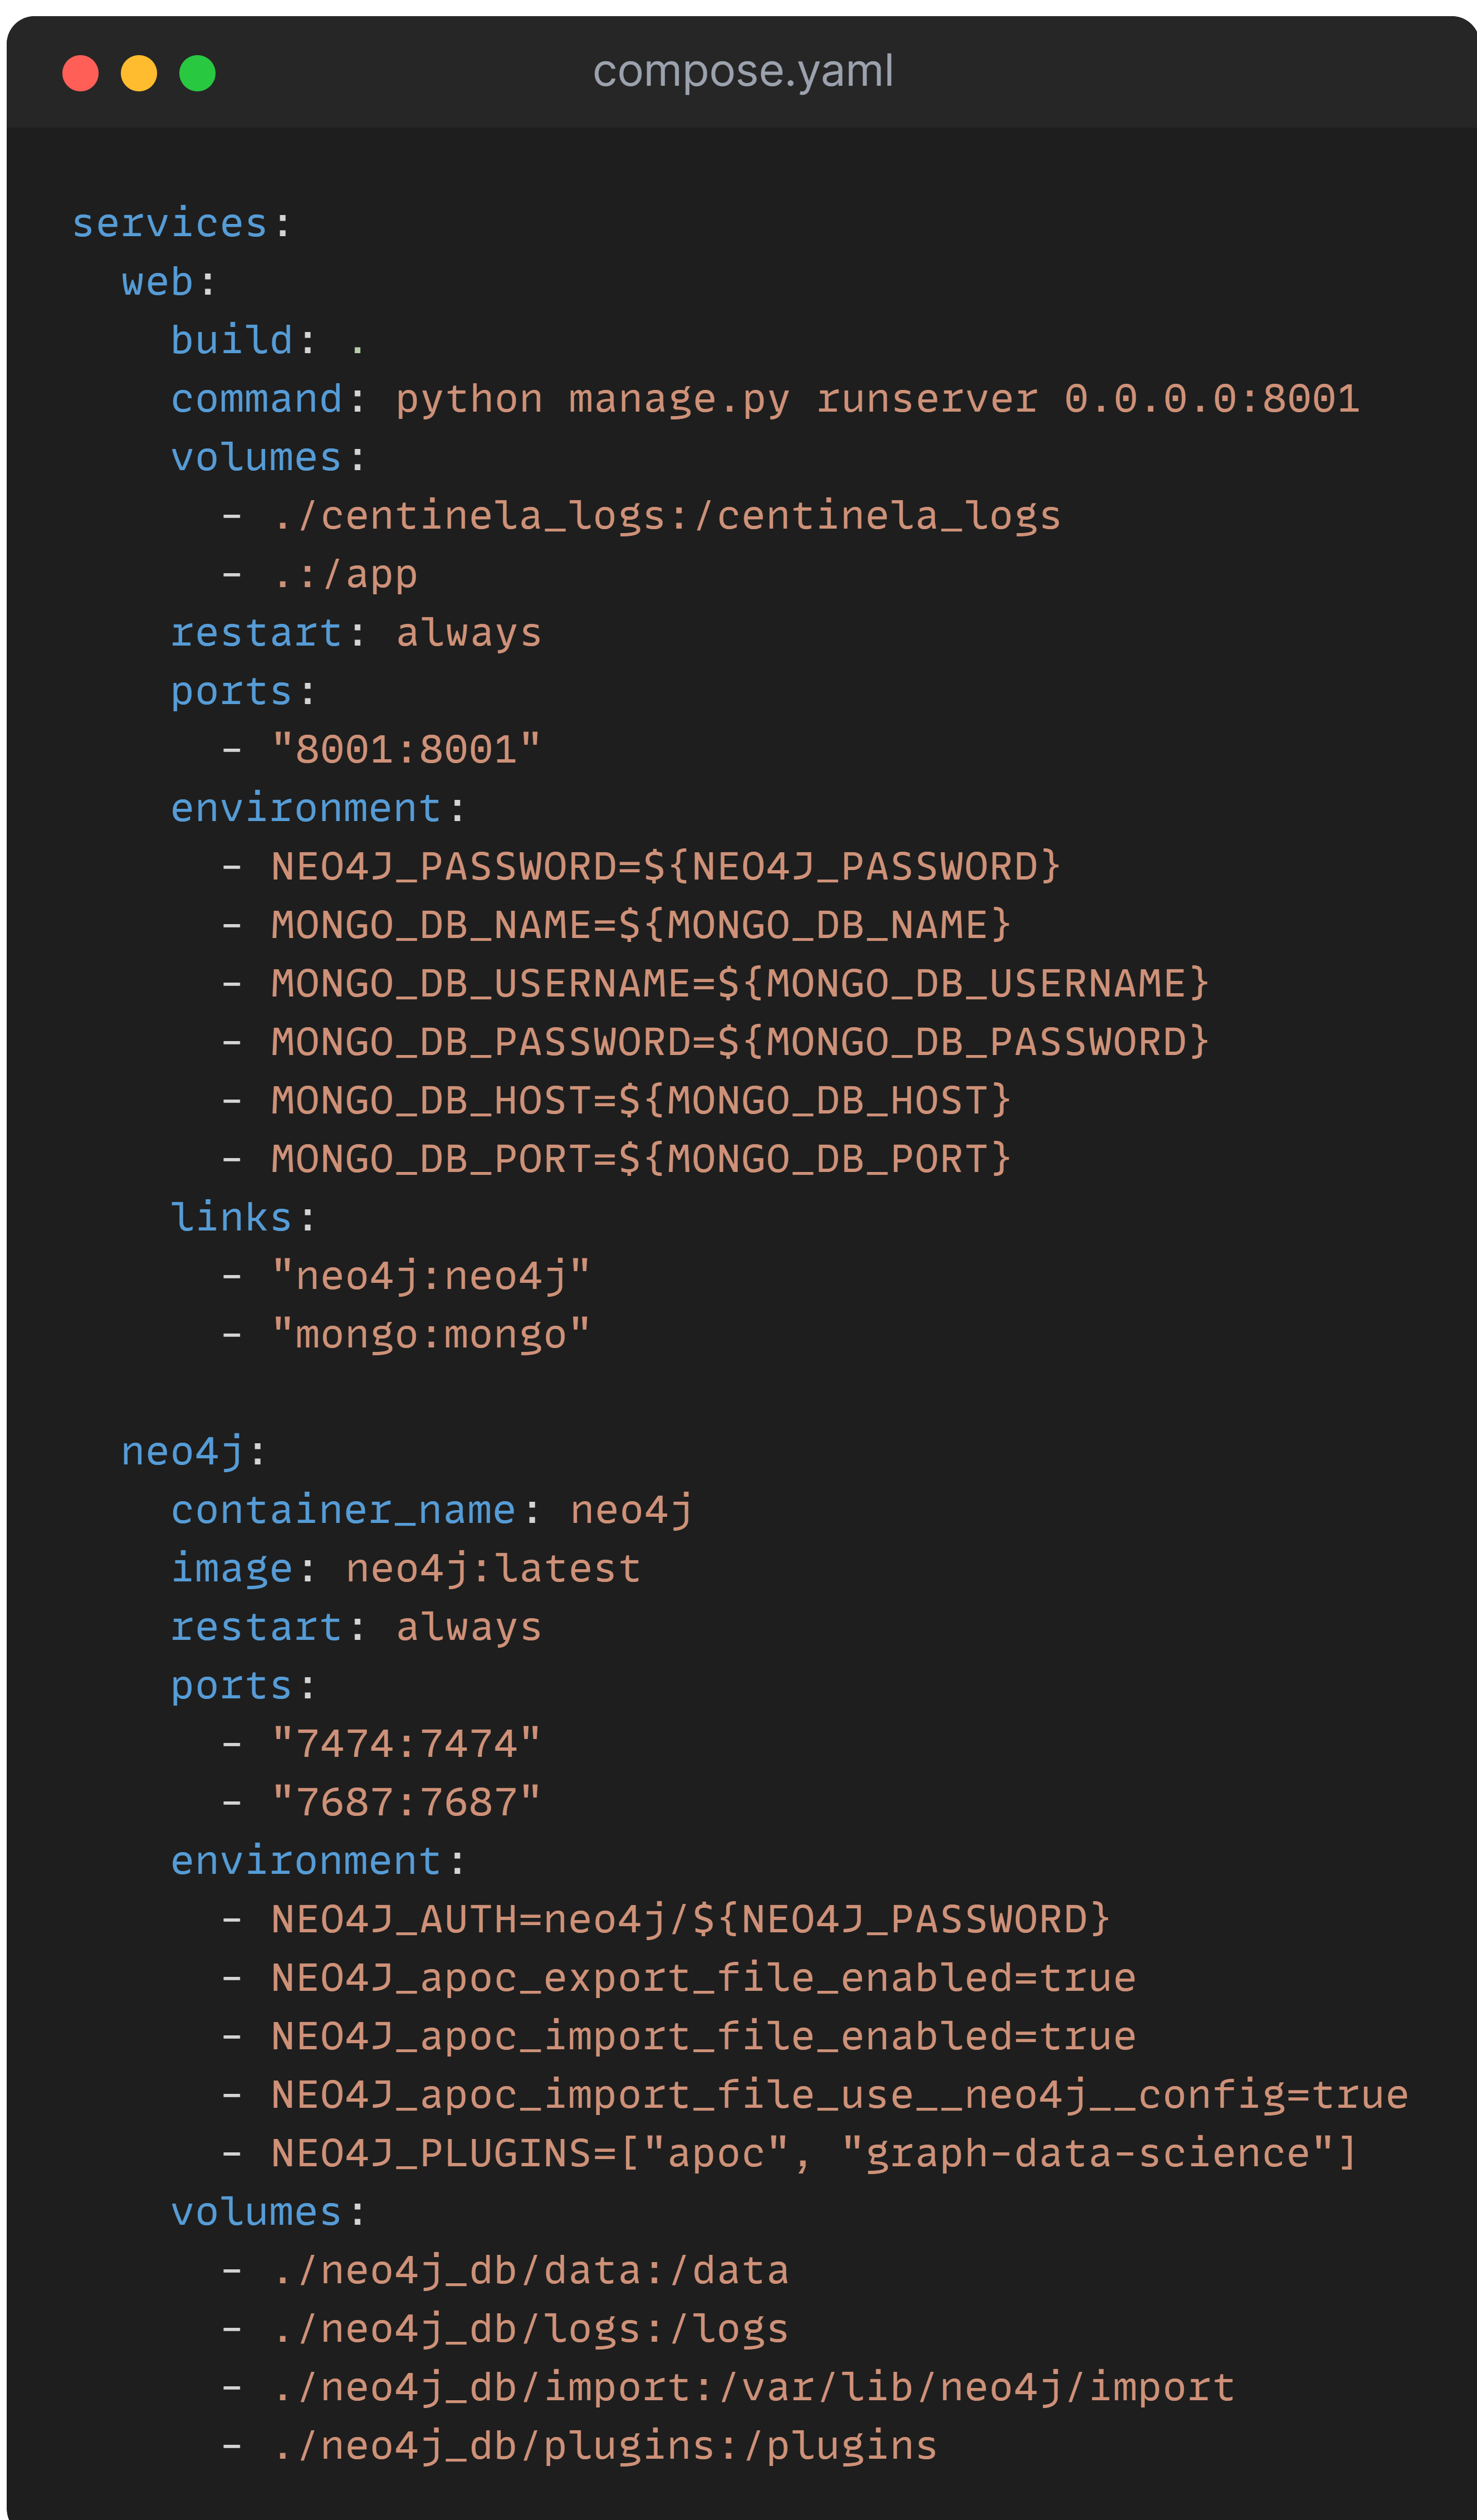
\includegraphics[scale=0.12]{../02Figures/02Chapter/Sprints/Sprint-3/compose-yaml.png}
    \caption{Archivo Docker Compose}
    \label{fig:docker-compose}
\end{figure}

Una vez configurado los archivos de Docker y Docker Compose,
se procedió a levantar los contenedores con el comando \textit{docker-compose up --build}.
Este comando se encarga de construir y levantar los servicios de la aplicación y la base de datos.
Para verificar que los contenedores se encuentran en ejecución se utiliza el comando \textit{docker ps}.
En la Figura \ref{fig:docker-ps} se muestra la salida del comando \textit{docker ps}.

\begin{figure}[H]
    \centering
    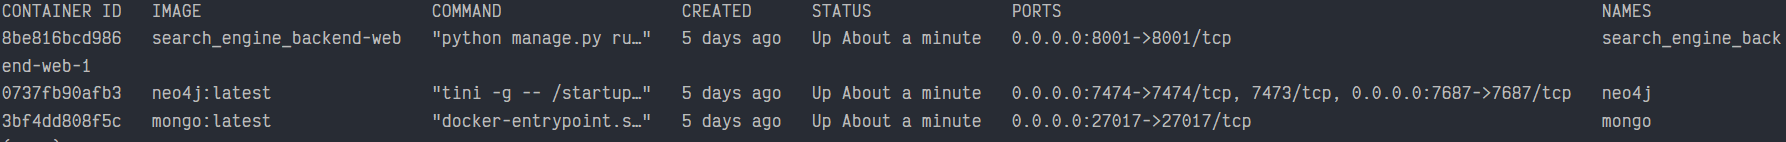
\includegraphics[scale=0.4]{../02Figures/02Chapter/Sprints/Sprint-3/docker-ps.png}
    \caption{Sialida del comando docker ps}
    \label{fig:docker-ps}
\end{figure}

Con el entorno de desarrollo configurado. Se procedió a la creación de las aplicaciones de Django.
Django denomina aplicaciones a un conjunto de funcionalidades que se pueden reutilizar en diferentes proyectos.
En este caso se crearon 3 aplicaciones \textit{dashboards}, \textit{scopus\_integration} y \textit{search\_engine}. Las mismas que se pueden observar en la Figura \ref{fig:django-apps}.
\begin{figure}[H]
    \centering
    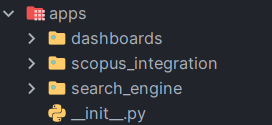
\includegraphics[scale=1]{../02Figures/02Chapter/Sprints/Sprint-3/django-apps.png}
    \caption{Aplicaciones de Django}
    \label{fig:django-apps}
\end{figure}

Las mismas que tendrán la estructura de carpetas en base a Arquitectura Hexagonal, como se menciono en la Sección \ref{chapter02-section02-sprint0}.
Cada aplicación tendrá su propia capa de dominio, aplicación e infraestructura.
Así como cada una tendrá una función específica en la aplicación, \textit{dashboards} se encargara de la visualización de los datos, \textit{scopus\_integration} de la integración con Scopus y \textit{search\_engine} de la funcionalidad del motor de busqueda.

Una vez finalizada la creación de las aplicaciones,  procedió a hacer el rediseño de la base de datos
previo a la implementación de los modelos en Neonmodel. Como se menciono en la Sección \ref{section:introduction-sprint-3} se tomo como base el diseño en Neo4j propuesto en Resnet.
Únicamente se agrego nuevos atributos a los nodos y relacione existentes.
Mas específicamente se agregaron atributos al nodo de \textit{Autor} y a la relación \textit{COAUTHORED}.
En la Figura \ref{fig:neo4j-model} se muestra el diseño de la base de datos.

\begin{figure}[H]
    \centering
    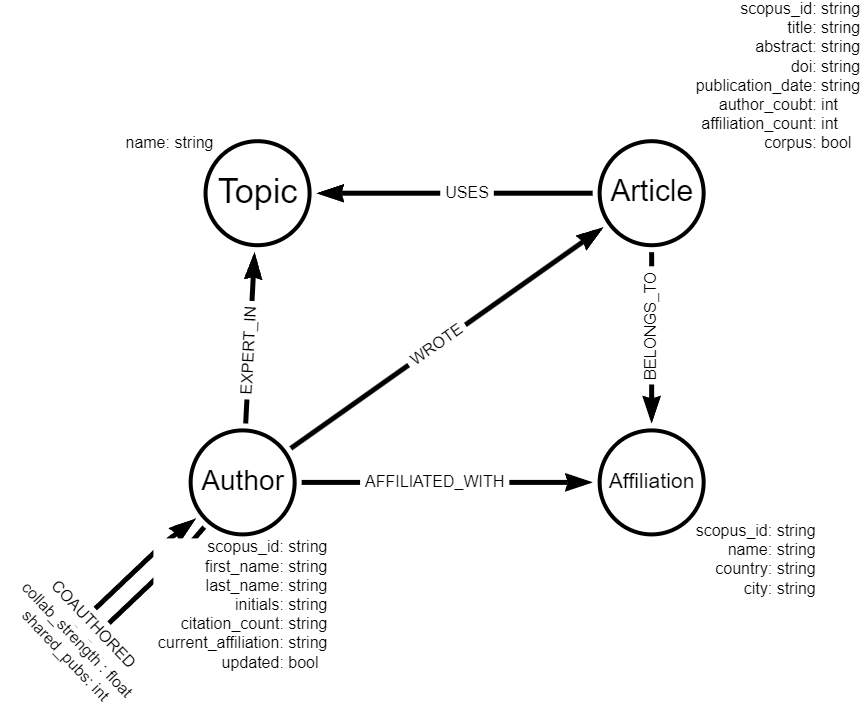
\includegraphics[scale=0.5]{../02Figures/02Chapter/Sprints/Sprint-3/centinela-graph.design-light.png}
    \caption{Modelo de la base de datos }
    \label{fig:neo4j-model}
\end{figure}

Con estas actualizaciones en el modelo, se procedió a la implementación de los mismos en Neomodel.
Como se menciono en el Sprint 0, para el desarrollo de la aplicación
se utilizara Arquitectura Hexagonal. Bajo este enfoque se crearon los modelos de la base de datos en la capa de dominio.
En la Figura \ref{fig:domain-layer} se muestra la capa de dominio de la aplicación que se encargara del motor de búsqueda.

\begin{figure}[H]
    \centering
    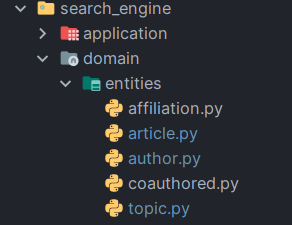
\includegraphics[scale=0.9]{../02Figures/02Chapter/Sprints/Sprint-3/domain-layer.png}
    \caption{Capa de dominio de la aplicación}
    \label{fig:domain-layer}
\end{figure}

Basándonos en el diseño de la base de datos que se muestra en la Figura \ref{fig:neo4j-model},
se muestra el modelo \textit{Author} implementado con Neomodel en la Figura \ref{fig:author-model}.
En terminos generales para asegurar la integridad de los datos se hace uso  de las restricciones de unicidad de Neomodel, con el tipo de dato \textit{UniqueIdProperty}.
Esto será de gran utilidad para evitar la creación de nodos duplicados en la base de datos.
Asimismo se utilizan las propiedades de tipo \textit{Relationship} y \textit{RelationshipTo} para definir las relaciones entre los nodos.

\begin{figure}[H]
    \centering
    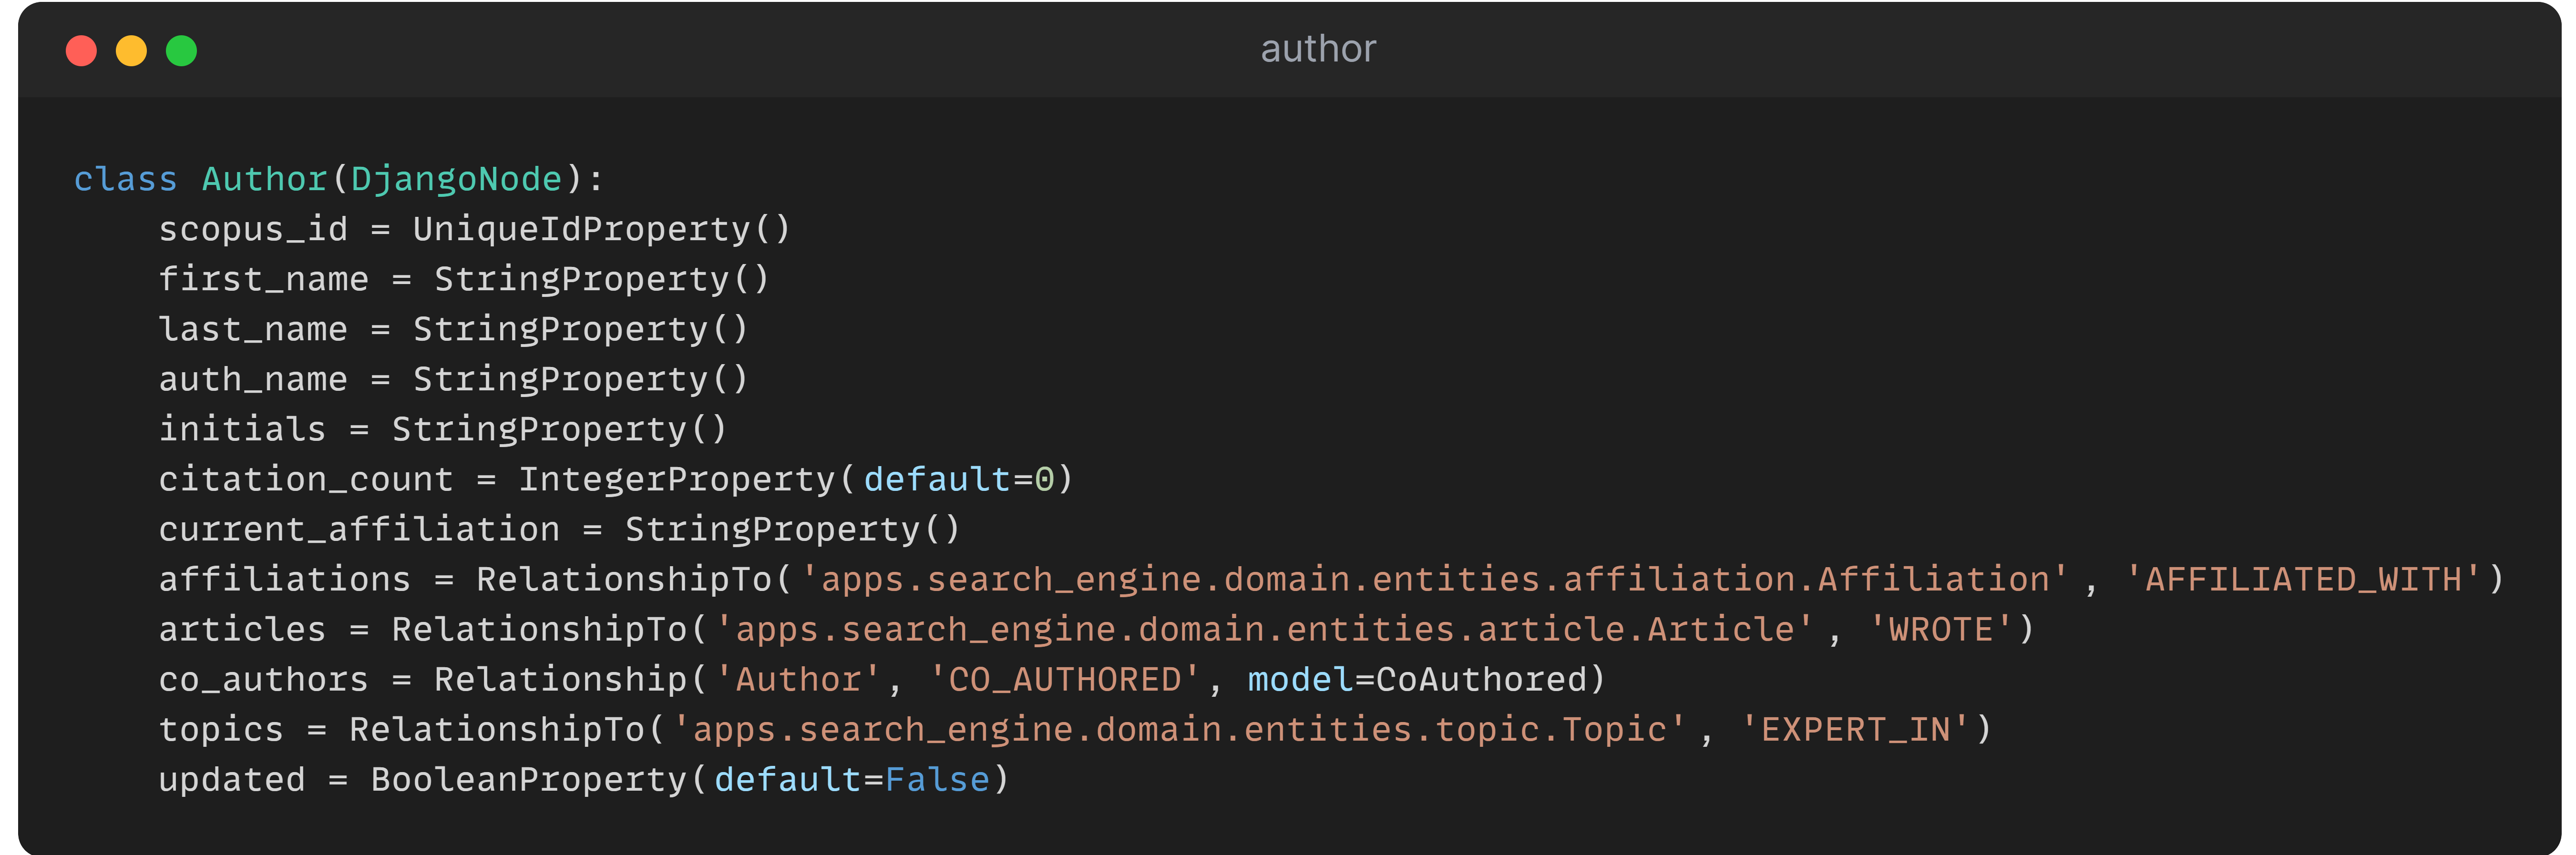
\includegraphics[scale=0.12]{../02Figures/02Chapter/Sprints/Sprint-3/author-neomodel.png}
    \caption{Modelo Author implementado con Neomodel}
    \label{fig:author-model}
\end{figure}

Finalmente la migración de estos modelos a la base de datos se realiza con el comando \texttt{python manage.py install\_labels}.
Aunque este comando es opcional es recomendable ejecutarlo para asegurar que los modelos se encuentren en la base de datos, o si en su defecto se requiere hacer una actualización de los modelos.

Siguiendo la Arquitectura Hexagonal, se procedió a implementar la funcionalidad de búsqueda de autores.
Para ello, se creó el repositorio AuthorRepository en la capa de dominio, encargado de definir los métodos necesarios para la búsqueda de autores.

El uso del patrón de diseño Repository garantiza la separación entre la lógica de negocio y la lógica de persistencia. Posteriormente, en la capa de aplicación, se implementará la lógica de negocio correspondiente a cada una de las funciones definidas en el repositorio.

En la Figura \ref{fig:author-repository} se muestra un extracto del repositorio \textit{AuthorRepository} con algunos de los métodos que nos servirán para la búsqueda de autores.

\begin{figure}[H]
    \centering
    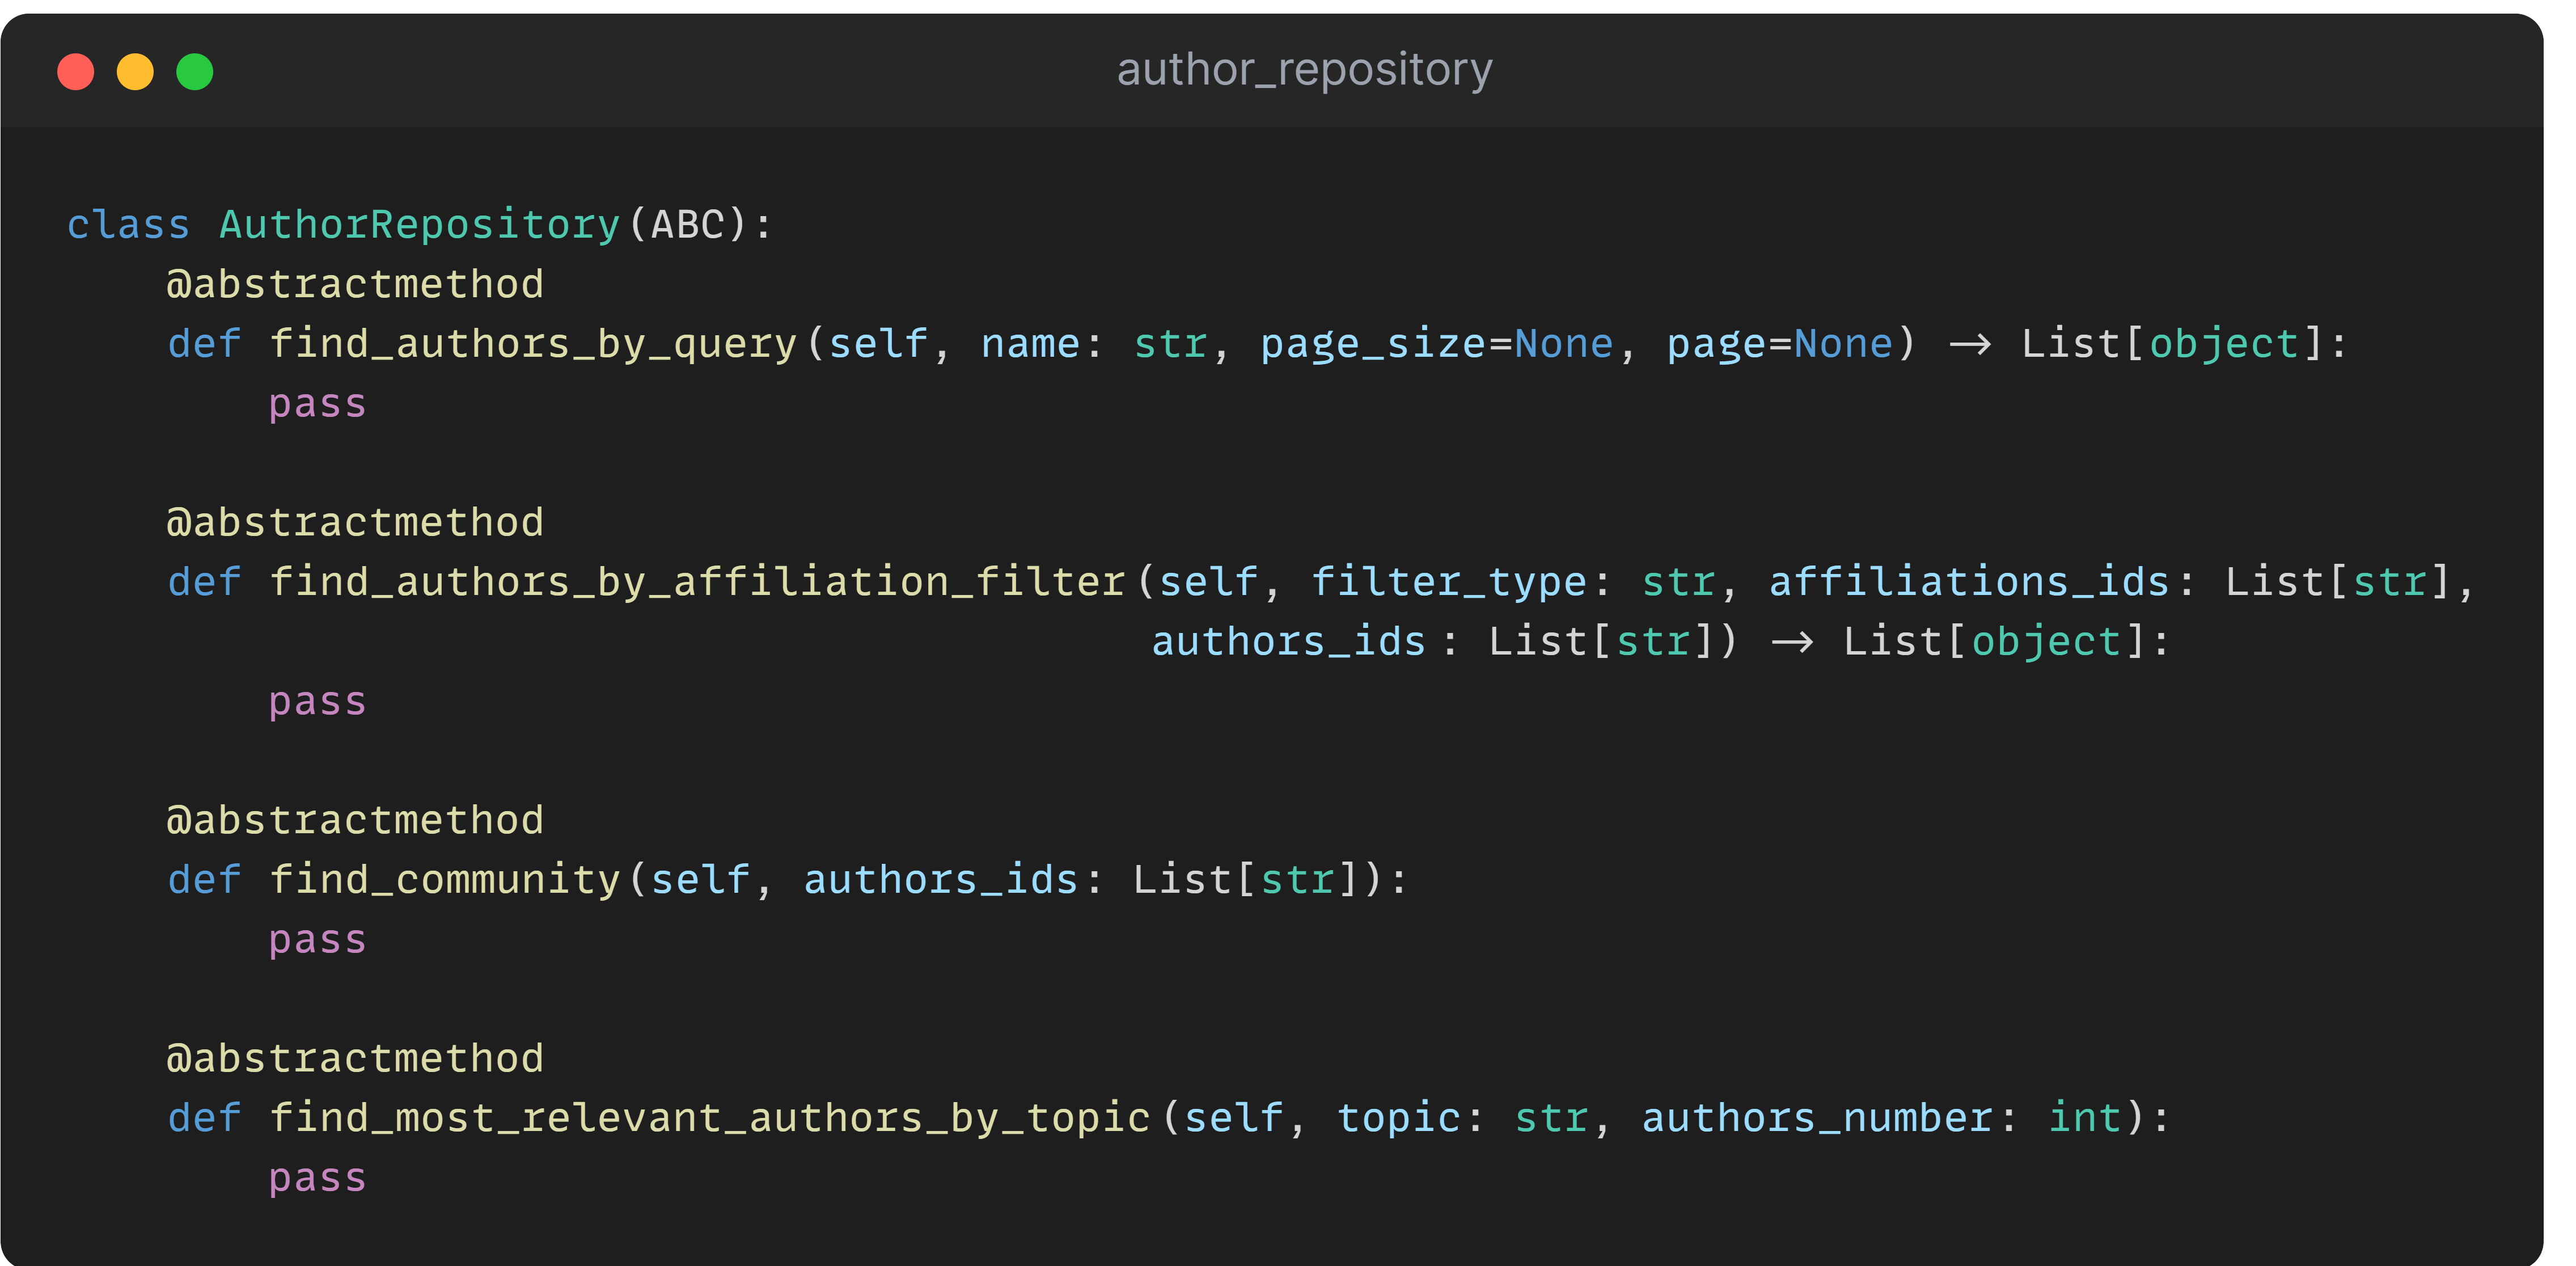
\includegraphics[scale=0.13]{../02Figures/02Chapter/Sprints/Sprint-3/author-repository.png}
    \caption{Repositorio AuthorRepository}
    \label{fig:author-repository}
\end{figure}

Una vez definidos los repositorios pasamos a la capa de aplicación, en la cual se implementa la lógica de negocio correspondiente a cada uno de los métodos definidos en el repositorio.
La Figura \ref{fig:author-service} muestra un extracto del servicio \textit{AuthorService} el mismo que hereda de la clase \textit{AuthorRepository} con la implementación de la función \textit{find\_authors\_by\_query}.

\begin{figure}[H]
    \centering
    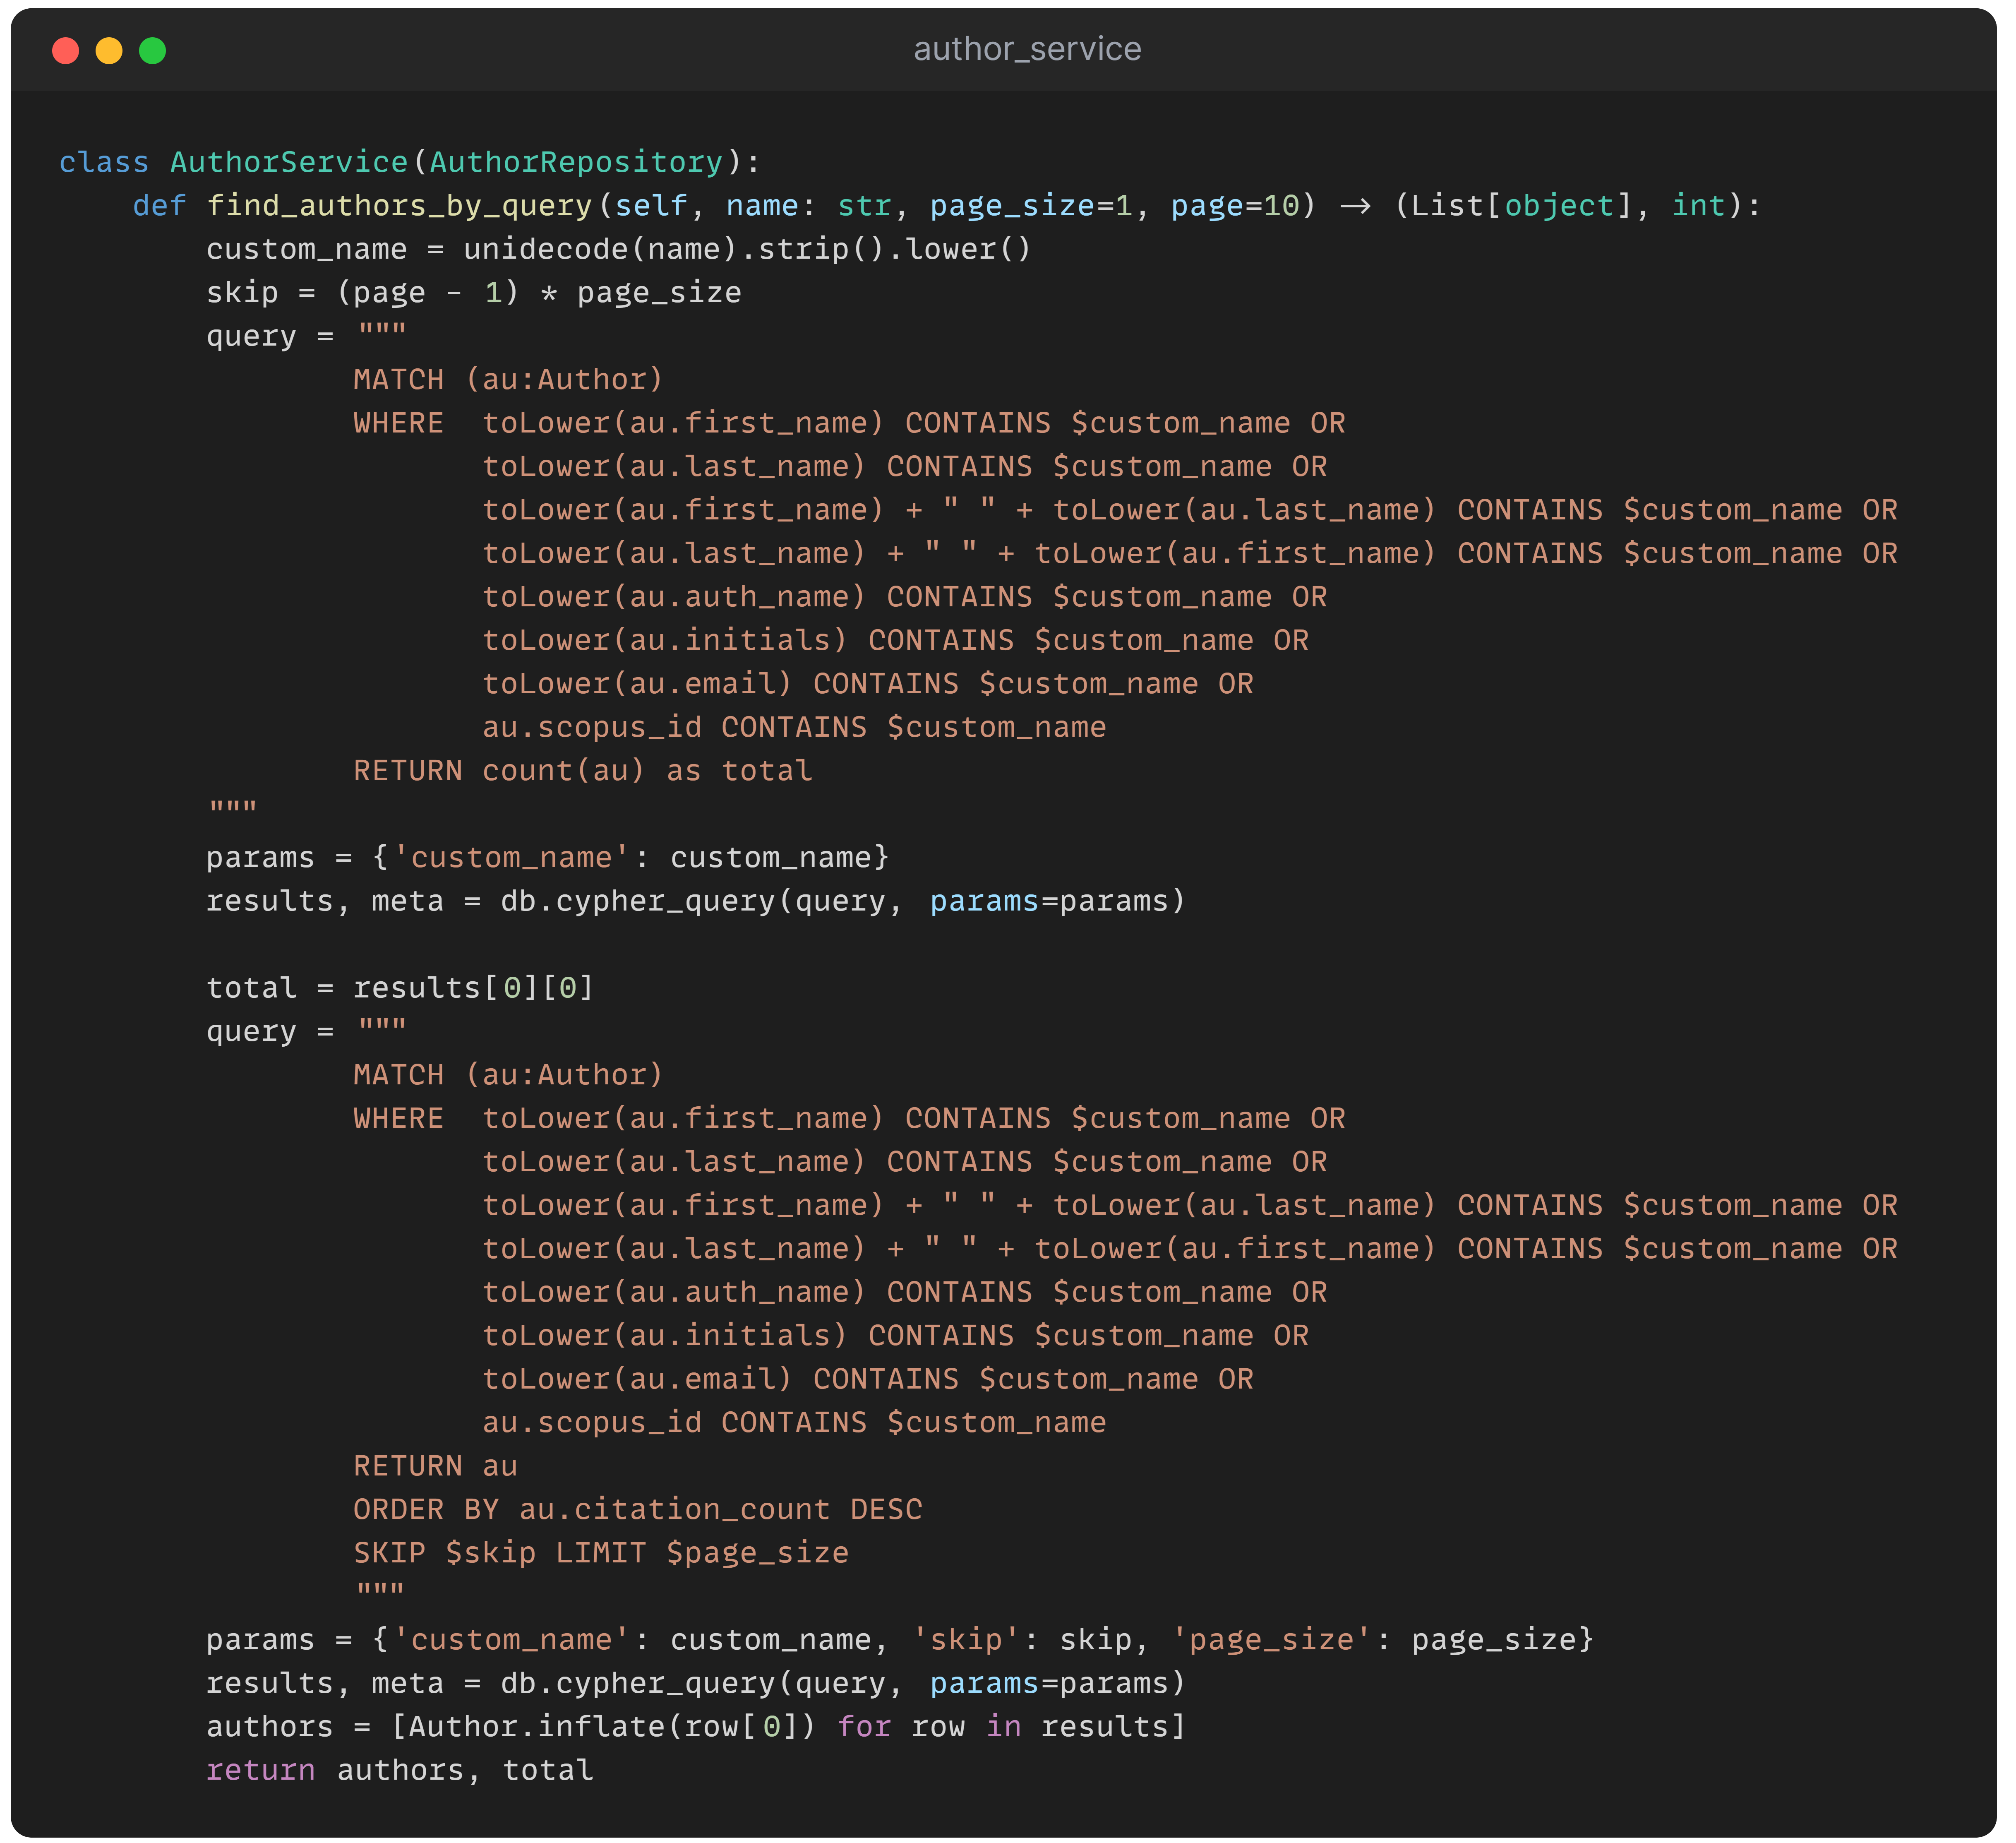
\includegraphics[scale=0.11]{../02Figures/02Chapter/Sprints/Sprint-3/author-service.png}
    \caption{Servicio AuthorService}
    \label{fig:author-service}
\end{figure}


Dado que en este caso se está utilizando una base de datos orientada a grafos,
se empleó el lenguaje de consulta Cypher para realizar la búsqueda de autores.
Usar Cypher permite aprovechar las ventajas de las bases de datos orientadas a grafos,
como la rapidez en la consulta de datos y la facilidad para encontrar relaciones entre los nodos.

Sin embargo, existe el riesgo de Cypher Injection, por lo que es fundamental tener
cuidado al construir las consultas. Para todas las consultas,
se utilizó el método \textit{cypher\_query} de Neomodel, que permite ejecutar consultas Cypher directamente en la base de datos,
enviando los parámetros no en la cadena de texto sino como argumentos de la función.
Esto evita la inyección de Cypher en la base de datos,
sanitizando las consultas y protegiéndolas de posibles inyecciones de Cypher.

Una vez con el servicio listo se procedió a la implementación del caso de uso \textit{FindAuthorsByQuery} en la capa de aplicación.
En la Figura \ref{fig:find-authors-by-query} se muestra el caso de uso que se encargara de llamar a los repositorios necesarios para la busqueda de autores.

\begin{figure}[H]
    \centering
    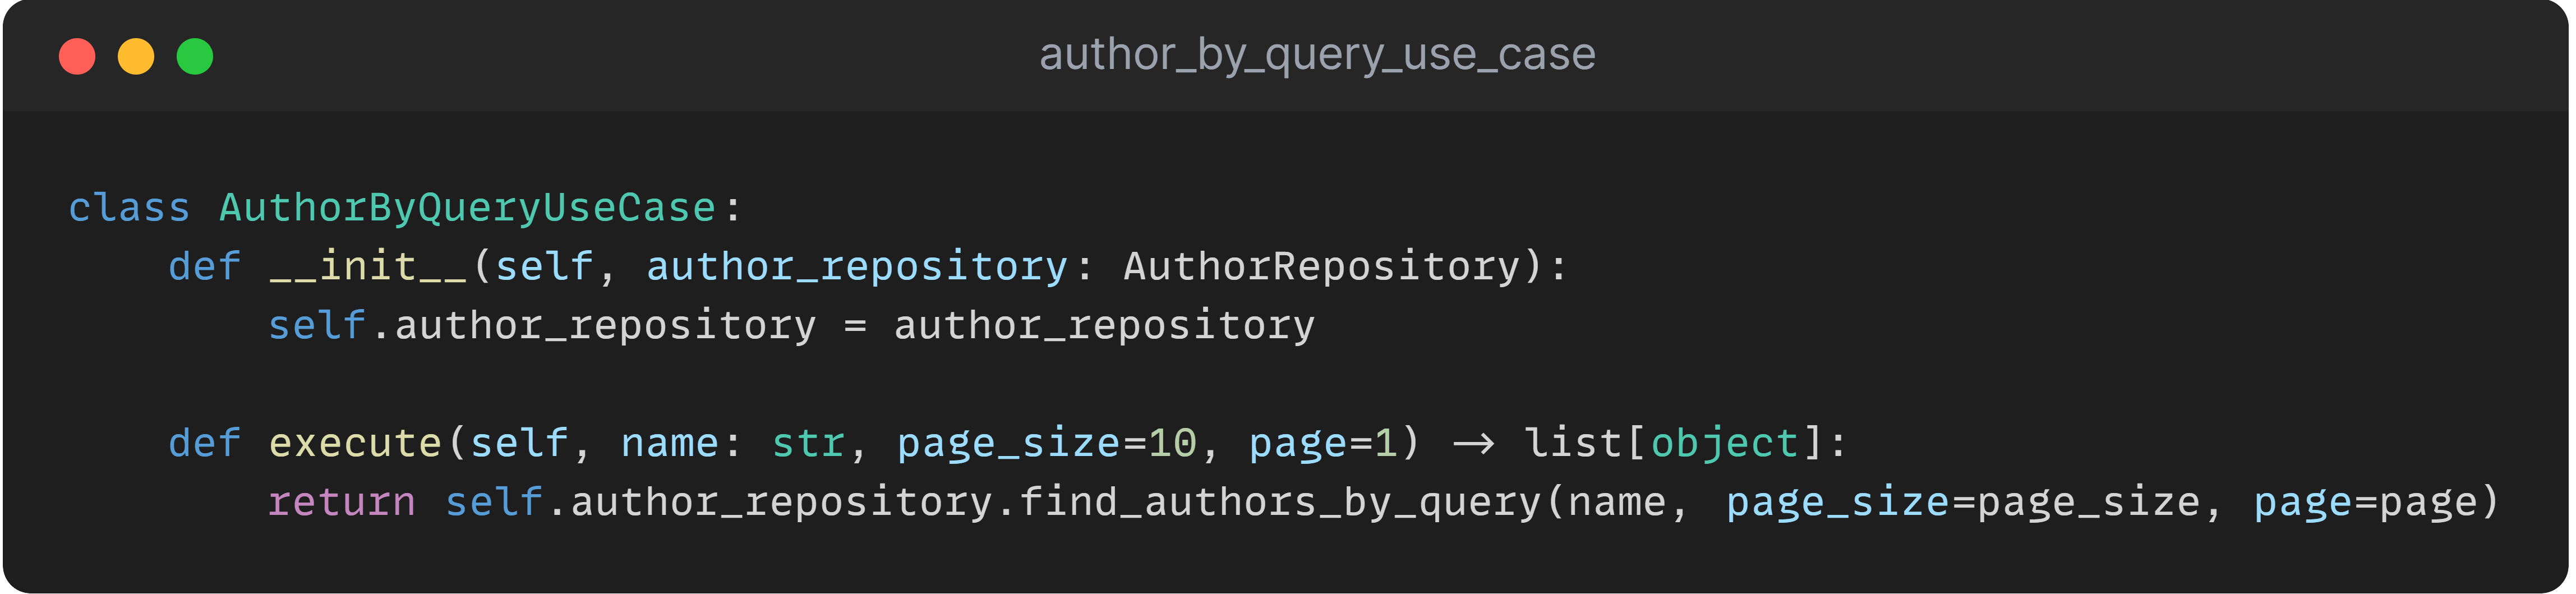
\includegraphics[scale=0.11]{../02Figures/02Chapter/Sprints/Sprint-3/author-by-query-use-case.png}
    \caption{Caso de uso FindAuthorsByQuery}
    \label{fig:find-authors-by-query}
\end{figure}

A continuación se procedió a la implementación de la capa de infraestructura.
Esta capa se va a encargar de la comunicación con el exterior de la aplicación, en este caso con la API REST.
Para ello se creó la vista \textit{AuthorViews} que se encargará de recibir las peticiones HTTP y llamar a los casos de uso correspondientes.
En la Figura \ref{fig:author-views} se muestra un extracto de la vista \textit{AuthorViews} con la implementación del caso de uso \textit{FindAuthorsByQuery}.
Como se puede observar, la vista únicamente se encarga de recibir la petición HTTP y llamar al caso de uso correspondiente. No maneja la lógica de negocio.
Esto permite que la vista sea independiente de la lógica de negocio y de la lógica de persistencia. De esta manera, se garantiza la separación de responsabilidades y se facilita la reutilización de código, logrando que la aplicación sea más mantenible y escalable.
\begin{figure}[H]
    \centering
    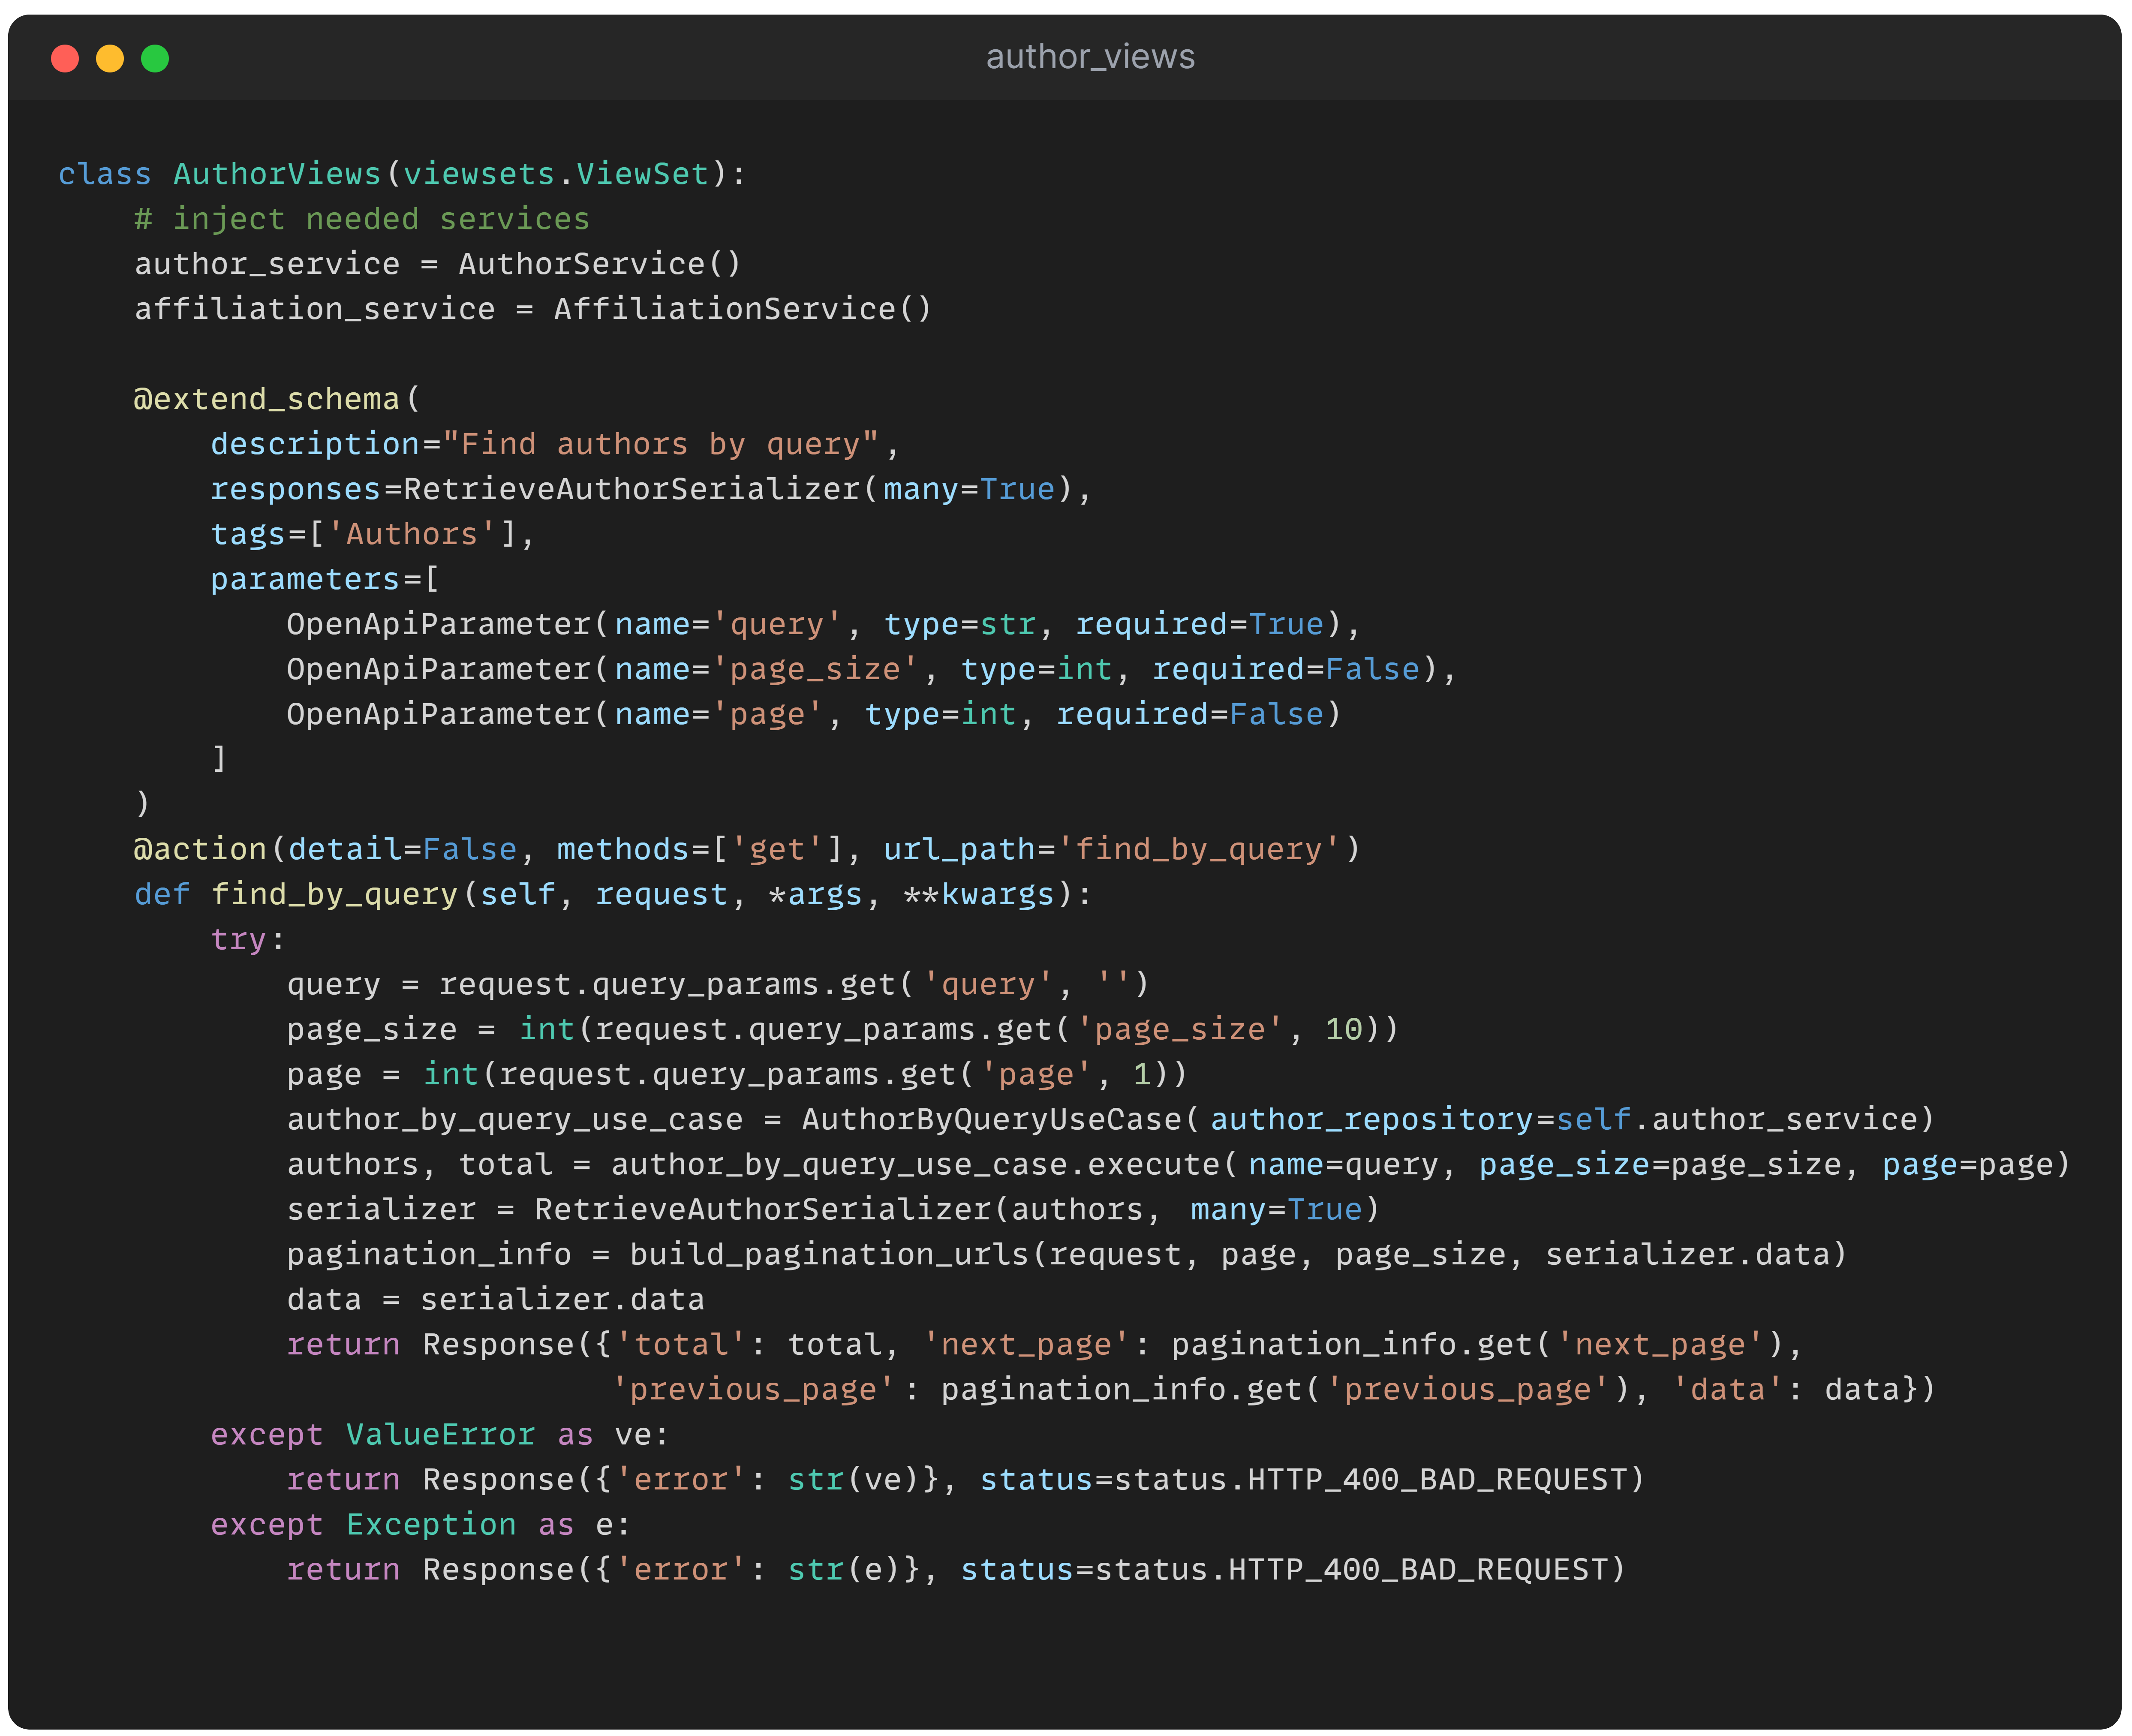
\includegraphics[scale=0.085]{../02Figures/02Chapter/Sprints/Sprint-3/author-views.png}
    \caption{Vista AuthorViews}
    \label{fig:author-views}
\end{figure}

También se implemento la serialización de los datos en la capa de infraestructura.
Para ello se creo el serializador \textit{AuthorSerializer} que se encargara de serializar los datos de los autores.
Ademas, se utilizo Swagger para documentar la API REST. En la Figura \ref{fig:author-views} se puede visualizar el decorador \footnote{
    Un decorador es una función que toma otra función y extiende su funcionalidad sin modificarla.} \textit{extend\_schema} que permite la documentación automática de la API, en este caso se documenta el endpoint \textit{find\_by\_query}.
El resultado de la documentación se muestra en la Figura \ref{fig:swagger}. La cual tiene una interfaz gráfica que permite probar los endpoints de la API.

\begin{figure}[H]
    \centering
    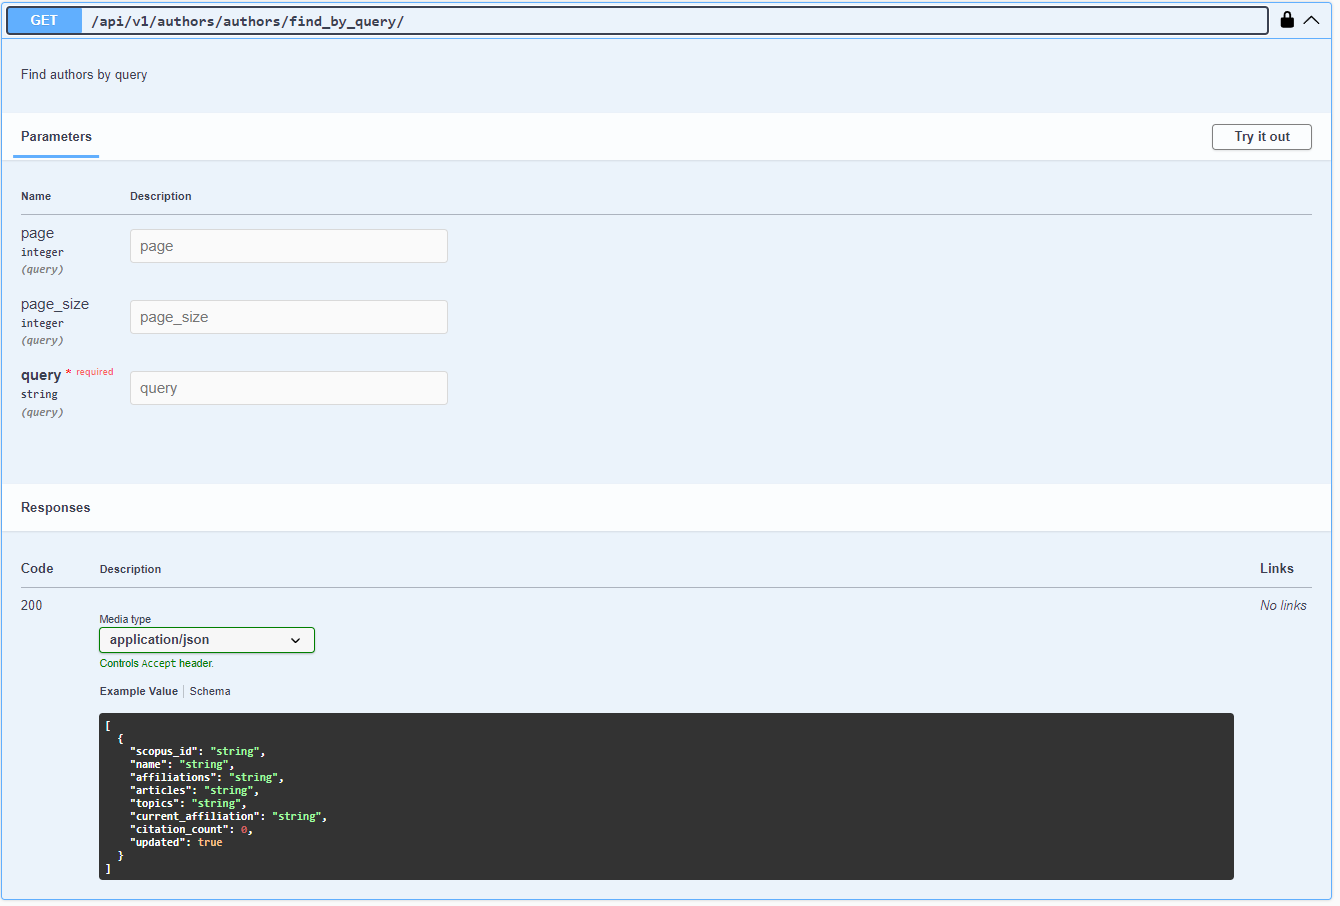
\includegraphics[scale=0.5]{../02Figures/02Chapter/Sprints/Sprint-3/swagger-ui.png}
    \caption{Documentación de la API con Swagger}
    \label{fig:swagger}
\end{figure}

Todo lo descrito anteriormente para la implementación de la funcionalidad de búsqueda de autores se puede resumir con un diagrama de secuencia.
En la Figura \ref{fig:sequence-diagram-authors-by-query} se muestra el diagrama de secuencia de la funcionalidad de búsqueda de autores.
En resumen con este diagrama de secuencia se puede observar el flujo de la aplicación. La petición HTTP llega a la vista \textit{AuthorViews}, la vista llama al caso de uso \textit{FindAuthorsByQuery}, el caso de uso llama al repositorio \textit{AuthorRepository} y este a su vez ejecuta la consulta en la base de datos.
También podemos distinguir las capas por sus colores por ejemplo la capa de dominio esta representada en color naranja, la capa de aplicación en color amarillo y la capa de infraestructura en color verde.
A partir de este punto se representará únicamente el flujo de la aplicación, sin entrar en detalles de la implementación.
\begin{figure}[H]
    \centering
    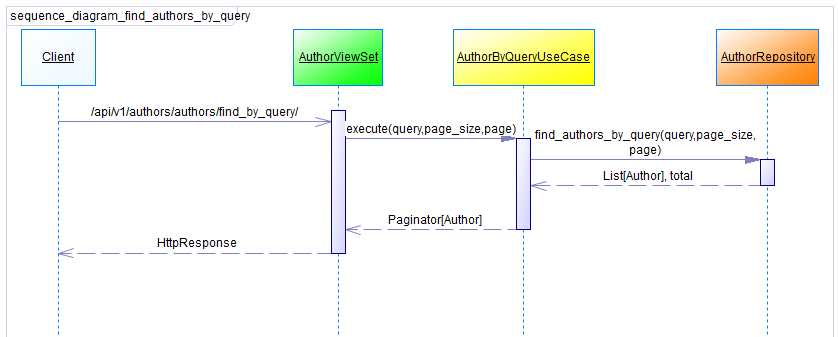
\includegraphics[scale=0.9]{../02Figures/02Chapter/Sprints/Sprint-4/sequence_diagram_find_authors_by_query.png}
    \caption{Diagrama de secuencia de la funcionalidad de búsqueda de autores}
    \label{fig:sequence-diagram-authors-by-query}
    
\end{figure}


\subsection{Revisión y Retrospectiva}
En la revision del Sprint 3 se verificó que se cumplieran los criterios de aceptación de las historias de usuario seleccionadas.
Se comprobó que la funcionalidad de búsqueda de autores funcionara correctamente y que la documentación de la API REST estuviera actualizada.
Además, se verificó que los modelos de la base de datos se encontraran en la base de datos.
En la Figura \ref{fig:neo4j-browser} se muestra la base de datos con los nodos y relaciones creados.

\begin{figure}[H]
    \centering
    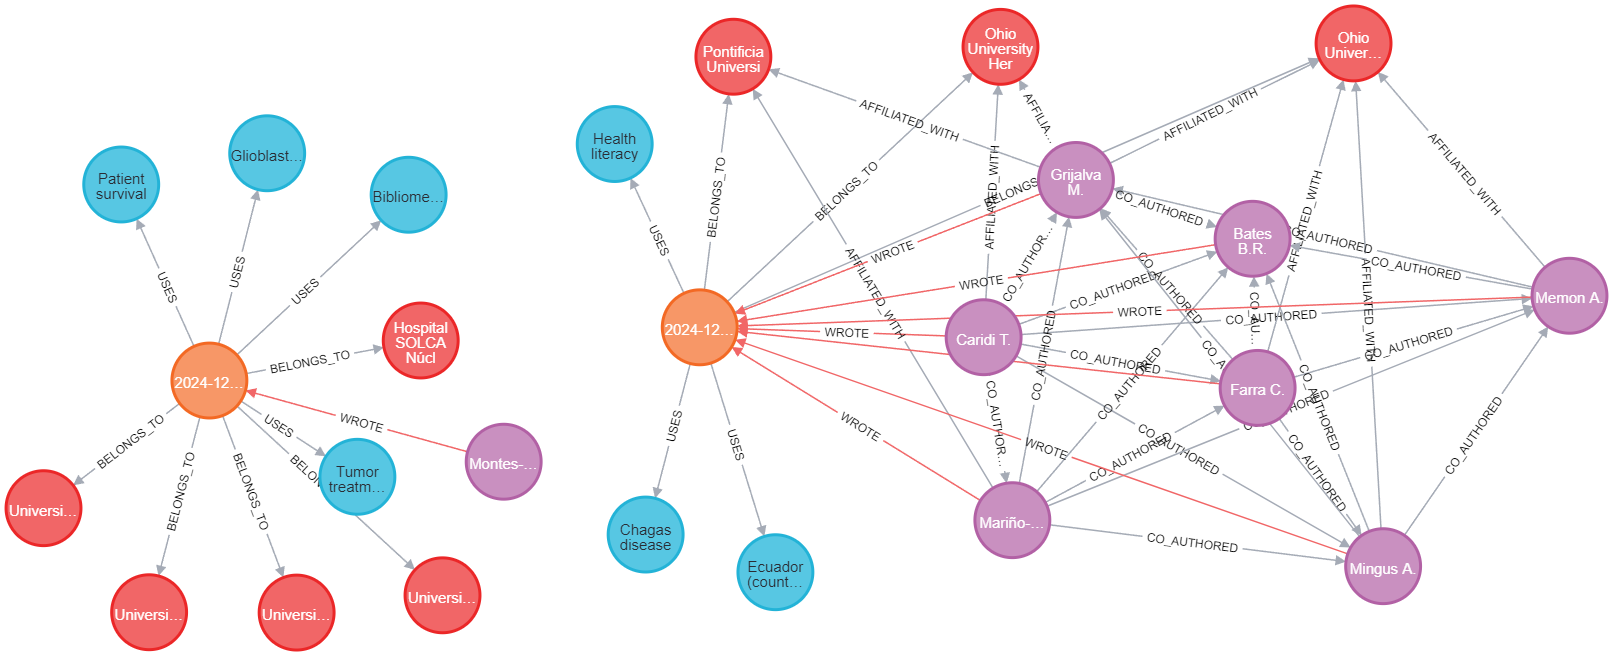
\includegraphics[scale=0.2]{../02Figures/02Chapter/Sprints/Sprint-3/graph-database.png}
    \caption{Base de datos Neo4j}
    \label{fig:neo4j-browser}
\end{figure}

Se considera que se cumplió con los objetivos planteados para este sprint, ya que se logró implementar la funcionalidad de búsqueda de autores y se rediseñó la base de datos en Neo4j utilizando Neomodel.
Además, se logró levantar el ambiente de desarrollo con Docker y Docker Compose.

Sin embargo, se presentaron algunos problemas durante el desarrollo de las tareas asignadas.
Uno de los problemas más significativos fue la falta de documentación de Neomodel, lo que dificultó la implementación de los modelos en la base de datos.
La falta de datos de prueba también fue un problema, ya que se tuvo que trabajar con datos ficticios para realizar las pruebas de la funcionalidad de búsqueda de autores.


\section{Sprint 4}
\label{chapter02-section02-sprint4}
\subsection{Introducción}
El cuarto sprint tiene como objetivo alcanzar el estado final de Resnet,
es decir, lograr que Centinela esté completamente funcional y lista para ser
utilizada por los usuarios. En el contexto del motor de búsqueda,
se espera que  Centinela sea capaz de realizar las búsquedas
que Resnet podía realizar en su estado final, alcanzando así el nivel de funcionalidad de la versión anterior.
\subsection{Objetivos}
\begin{itemize}
    \item Implementar la automatización para generar el Corpus y el Modelo de TF-IDF
    \item Implementar la funcionalidad de búsqueda de autores relevantes dado un tópico
    \item Implementar la funcionalidad de búsqueda de artículos relevantes dado un tópico
    \item Implementar la funcionalidad para obtener la red de coautoría de un autor
    \item Implementar la funcionalidad para obtener un Articulo dado su ID de Scopus
    \item Implementar la funcionalidad para obtener un Autor dado su ID de Scopus
\end{itemize}
\subsection{Planificación}
Para este sprint se terminaron las tareas que quedaron pendientes en el Sprint 1 (Ver sección \ref{chapter02-section02-sprint1})  y en el Sprint 2 (Ver sección \ref{chapter02-section02-sprint2}).
En la tabla \ref{C2T4:Historias de Usuario del Sprint 4} se presentan las historias de usuario que se abordarán en este sprint con sus respectivas tareas.
\begin{table}[!t]
    \centering
    \begin{tabular}{|p{2.5cm}|p{5cm}|p{6cm}|}
        \midrule
        \textbf{Identificador} & \textbf{Historia de Usuario}                                                                                                                                                                               & \textbf{Tareas} \\
        \hline
        HU-SE-01 & Como usuario no registrado deseo poder encontrar artículos relevantes dado un  tema de investigación para poder acceder rápidamente a información útil y actualizada que apoye mi estudio o trabajo        &
        \begin{compactitem}
            \item Generar el corpus \footnote{
                Conjunto de documentos que se utilizan para entrenar un modelo de \textit{Machine Learning} o \textit{Deep Learning}
            } de datos  
            \item Generar el modelo de TF-IDF a partir del corpus
            \item Crear el modelo de Artículo para la base de datos
            \item Implementar el filtro de artículos por año
            \item Crear un servicio de búsqueda de artículos
            \item Desarrollar un endpoint para manejar las solicitudes entrantes
        \end{compactitem}
        \\
        \hline
        HU-SE-04 & Como usuario no registrado quiero poder ver los artículos de un investigador para conocer su trabajo y las publicaciones en las que ha contribuido &
        \begin{compactitem}
            \item Implementar un endpoint para recuperar el perfil de un investigador y sus publicaciones
            \item Crear un servicio de búsqueda de investigadores y sus artículos
        \end{compactitem}
        \\
        \hline
        HU-SE-03 & Como usuario no registrado, deseo poder ver la red de coautoría de un autor para visualizar un grafo con los autores con los que ha colaborado, así como la fuerza de esas colaboraciones &
        \begin{compactitem}
            \item Implementar un endpoint para recuperar los datos de colaboración entre autores
            \item Crear un servicio que genere los datos del grafo de coautoría de un autor
        \end{compactitem}
        \\
        \hline
    \end{tabular}
    \caption{Historias de Usuario del sprint 4}
    \label{C2T4:Historias de Usuario del Sprint 4}
\end{table}


Los criterios de aceptación para las historias de usuario HU-SE-01, HU-SE-03 y HU-SE-04 han sido definidos y se pueden consultar en las siguientes figuras: Figura \ref{fig:aceptance-criteria-HU-SE-01}, Figura \ref{C2F2:Criterios de Aceptacion HU-SE-03} y Figura \ref{C2F2:Criterios de Aceptacion HU-SE-04}.
\subsection{Implementación}

Para la implementación de ciertas tareas en este Sprint, se optó por reutilizar el código de la versión anterior de ResNet, ya que se consideró más eficiente y rápido que comenzar desde cero.
La optimización de funcionalidades existentes no está incluida en el alcance de este componente.
Las funcionalidades que se reutilizarán son la generación del corpus y el modelo de TF-IDF,
dado que estas tareas son las más demandantes en términos de tiempo y se determinó que no era necesario reimplementarlas.
A estas funcionalidades solo se les añadirá una capa de infraestructura,
ya que la lógica de negocio ya está implementada en la versión anterior de ResNet.
Esto garantizará un punto de entrada para generar tanto el corpus como el modelo de TF-IDF,
permitiendo su utilización en las búsquedas de autores y artículos.

%% HU-SE-01
Tarea: \textit{HU-SE-01: Generar el corpus de datos}
Dado que las funcionalidades de buscar autores y artículos relevantes dependen del corpus de datos, y del modelo de TF-IDF, estas tareas se realizarán en primer lugar.
Para poder generar el corpus de datos, el endppoint \textit{/api/v1/generate-corpus/} se encargará de recibir la petición mediante el método POST.
Este llamara al caso de uso \textit{GenerateCorpusUseCase} que se encargará de generar de ejecutar la lógica de negocio para generar el corpus de datos.
El mismo que toma datos de Autores, Artículos, y Tópicos de la base de datos Neo4j para crear los documentos y almacenarlos en un archivo Pickle.
En la figura \ref{fig:sequence-diagram-generate-corpus} se muestra el diagrama de secuencia para la generación del corpus de datos.

\begin{figure}[H]
    \centering
    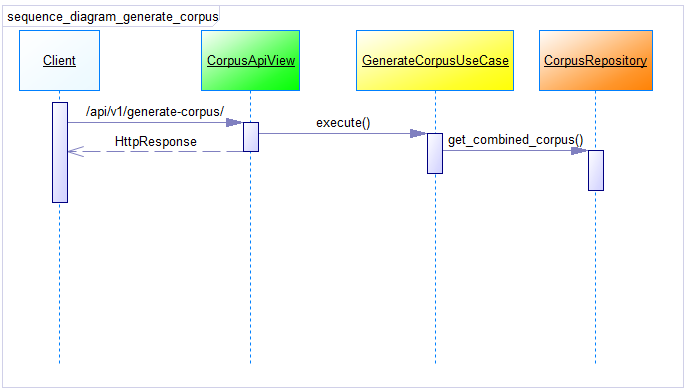
\includegraphics[scale=0.8]{../02Figures/02Chapter/Sprints/Sprint-4/sequence_diagram_generate_corpus.png}
    \caption{Diagrama de secuencia para la generación del Corpus}
    \label{fig:sequence-diagram-generate-corpus}
\end{figure}

Tarea: \textit{HU-SE-01: Generar el modelo de TF-IDF}
Una vez que el corpus de datos ha sido generado, se procederá a generar el modelo de TF-IDF.
Para ello, el endpoint \textit{/api/v1/generate-model/} se encargará de recibir la petición mediante el método POST.
Este llamara al caso de uso \textit{GenerateTfidfUseCase} que se encargará de ejecutar la lógica de negocio para generar el modelo de TF-IDF.
El mismo que toma el corpus de datos generado anteriormente y lo procesa para generar el modelo de TF-IDF, para guardar el modelo en un archivo Pickle.
En la figura \ref{fig:sequence-diagram-generate-tfidf} se muestra el diagrama de secuencia para la generación del modelo de TF-IDF.

\begin{figure}[H]
    \centering
    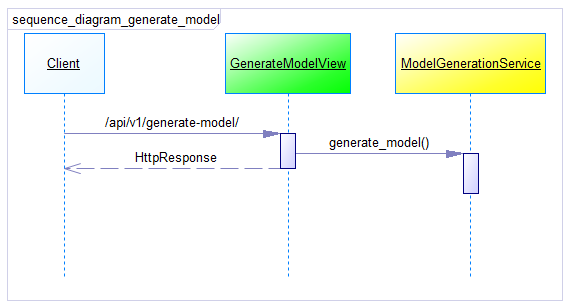
\includegraphics[scale=0.7]{../02Figures/02Chapter/Sprints/Sprint-4/sequence_diagram_generate_model.png}
    \caption{Diagrama de secuencia para la generación del Modelo de TF-IDF}
    \label{fig:sequence-diagram-generate-tfidf}
\end{figure}

Una vez que el corpus de datos y el modelo han sido generados se puede proceder a realizar las implementaciones tanto de autores relevantes como de artículos relevantes.
Para la funcionalidad de Artículos relevantes la ruta \textit{/api/v1/articles/most-relevant-articles-by-topic/} (POST) recibira en su cuerpo los siguientes datos:
\begin{itemize}
    \item query: El Tópico por el cual se desea buscar los Artículos relevantes
    \item size: El limite de Artículos que se desea obtener, por defecto es 10
    \item page: La pagina de Artículos que se desea obtener, por defecto es 1
    \item type: Si se desea incluir o excluir años de publicación
    \item years: Años de publicación a incluir o excluir
\end{itemize}
Este endpoint llamara al caso de uso \textit{GetMostRelevantArticlesByTopicUseCase} que se encargará de ejecutar la lógica de negocio para obtener los Artículos relevantes.
El proceso comienza tomando el tópico y pasándolo al modelo TF-IDF para identificar los IDs de los artículos relevantes. A continuación, se consulta la base de datos Neo4j para obtener los datos de esos artículos. Utilizando los parámetros de la petición, se buscan y retornan los artículos relevantes en una lista paginada, todo esto dentro de una respuesta Http.
En la figura \ref{fig:sequence-diagram-get-most-relevant-articles} se muestra el diagrama de secuencia para la obtención de los Artículos relevantes.

\begin{figure}[H]
    \centering
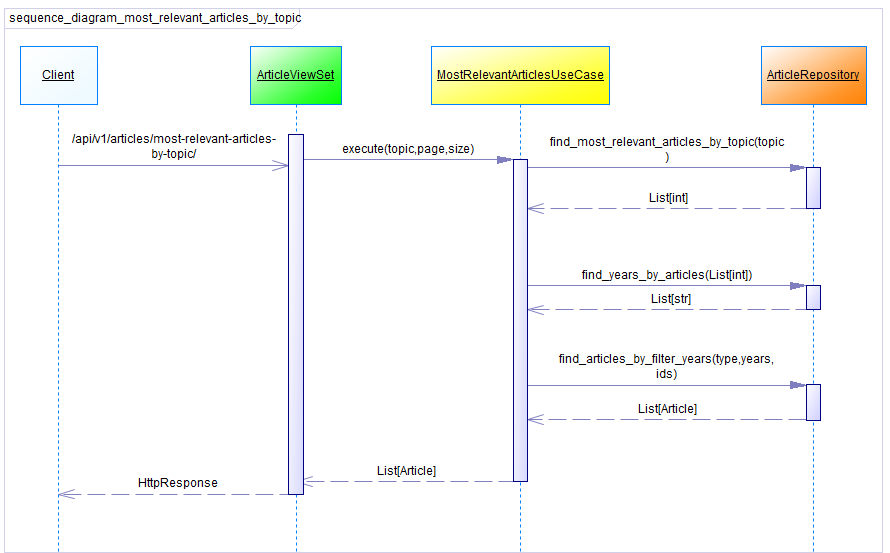
\includegraphics[scale=0.7]{../02Figures/02Chapter/Sprints/Sprint-4/sequence_diagram_most_relevant_articles_by_topic.png}
    \caption{Diagrama de secuencia para la obtención de los Artículos Relevantes}
    \label{fig:sequence-diagram-get-most-relevant-articles}
\end{figure}

%% HU-SE-03

HU-SE-03: Obtener la red de coautoría de un autor
Para la funcionalidad de obtener la red de coautoría de un autor, la ruta \textit{/api/v1/coauthors/coauthors/{id}/coauthors\_by\_id/} (GET) recibirá en su URL el ID del autor del cual se desea obtener la red de coautoría.
Este endpoint llamara al caso de uso \textit{GetCoauthorsByAuthorIdUseCase} que se encargará de ejecutar la lógica de negocio para obtener la red de coautoría de un autor.
El proceso comienza tomando el ID del autor y consultando la base de datos Neo4j para obtener los nodos (Autores) y links (collab\_strength) de la red de coautoría de ese autor. A continuación, se consultan los datos de esos coautores y se retornan en una respuesta Http.
En la figura \ref{fig:sequence-diagram-get-coauthors-by-author-id} se muestra el diagrama de secuencia para la obtención de la red de coautoría de un autor.
\begin{figure}[H]
    \centering
    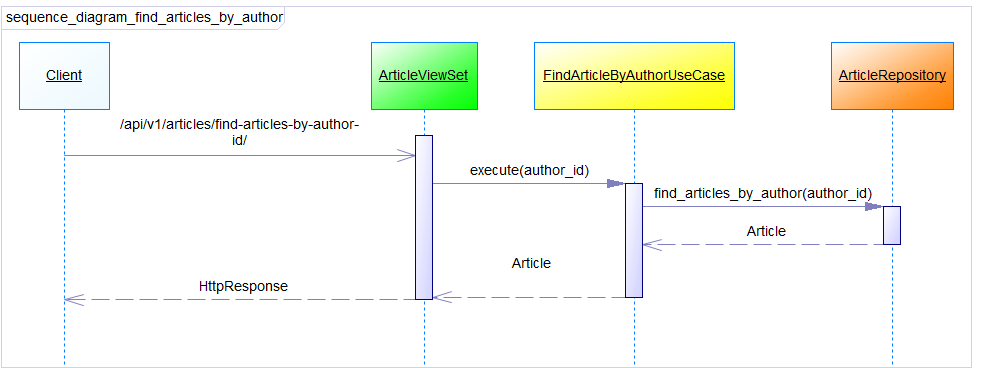
\includegraphics[scale=0.7]{../02Figures/02Chapter/Sprints/Sprint-4/sequence_diagram_find_articles_by_author.png}
    \caption{Diagrama de secuencia para la obtención de la red de coautoría de un autor}
    \label{fig:sequence-diagram-get-coauthors-by-author-id}
\end{figure}

%% HY-SE-04
HU-SE-03: Para obtener los Artículos en los que ha colaborado un autor, la ruta \textit{/api/v1/articles/find-articles-by-author-id/} (GET) recibirá en su URL el ID del autor del cual se desea obtener los articulos en los que ha colaborado.
Este endpoint llamara al caso de uso \textit{FindArticlesByAuthorIdUseCase} que se encargará de ejecutar la lógica de negocio para obtener los Artículos en los que ha colaborado un autor.
En la Figura \ref{fig:sequence-diagram-find-articles-by-author-id} se muestra el diagrama de secuencia para la obtención de los artículos en los que ha colaborado un autor.
\begin{figure}[H]
    \centering
    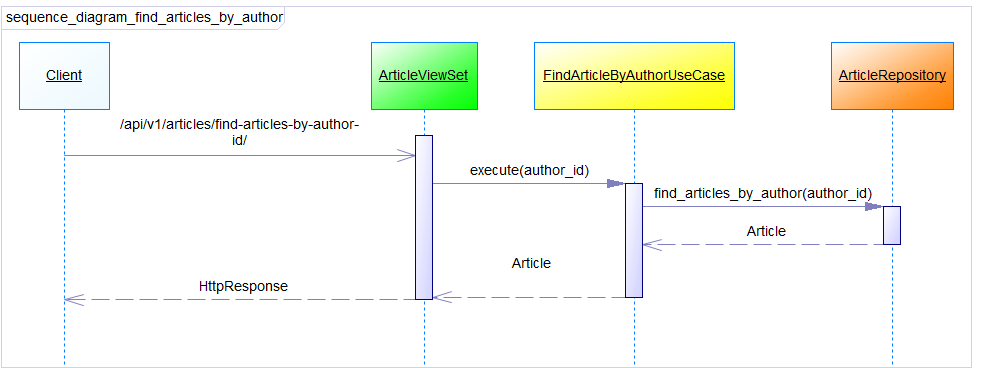
\includegraphics[scale=0.7]{../02Figures/02Chapter/Sprints/Sprint-4/sequence_diagram_find_articles_by_author.png}
    \caption{Diagrama de secuencia para la obtención de los Artículos en los que ha colaborado un autor}
    \label{fig:sequence-diagram-find-articles-by-author-id}
\end{figure}

\subsection{Revisión y Retrospectiva}
Al finalizar el sprint, se logró implementar las funcionalidades de búsqueda de autores y artículos relevantes, así como la obtención de la red de coautoría de un autor y la obtención de los artículos en los que ha colaborado un autor.
Mismas que habían quedado pendientes en los sprints anteriores. 
Así mismo, se logro evidenciar que la reutilización de código de la versión anterior de ResNet fue una buena decisión, ya que permitió acelerar el desarrollo de las funcionalidades.
También el uso de Arquitectura Hexagonal permitió diagramar de manera clara y concisa la implementación de las funcionalidades.

